\documentclass[a4paper,12pt]{article}
% \usepackage[a4paper,margin=3cm]{geometry}
\usepackage{graphicx}
\usepackage{fancyhdr}
\usepackage{xcolor}
\usepackage[table]{xcolor}
\usepackage{hyperref}
\usepackage{booktabs}
\usepackage{indentfirst}
\usepackage{subcaption}

\setlength{\arrayrulewidth}{0.5mm}
\setlength{\tabcolsep}{18pt}
\renewcommand{\arraystretch}{2.5}

\pagestyle{fancy}

\fancyhf{} 
\fancyhead[R]{\thepage}

\renewcommand{\contentsname}{\textcolor{teal}{Table of Contents}}

\begin{document}

\begin{titlepage}
    \begin{center}
        \vspace*{2cm}

        
\includegraphics[width=0.8\textwidth]{./img/slimg.png}\\[1cm]

        {\Huge \textbf{Smart Lock}}\\[0.5cm]
        {\textcolor{teal}{\Large A Cloud-Based Key}}\\[1.5cm]

        {\LARGE \textbf{}}\\[0.5cm]
        {\Large \textit{Nathaniel Laurente, Adam Wu, Neena Nguyen, Jackson Kennedy}}\\[2cm]

        {\Large \today}
    \end{center}
\end{titlepage}

\newpage
\pagenumbering{arabic}
\pagestyle{fancy}      



% BEGIN DOCUMENT -------------------------------------------------------------------------

% Executive Summary and Ethics Statement are the front matter (and don’t have section numbers). Start each section on a new page. First three pages are the title page, executive summary and the ethics statement. Then you have the table of contents.
\section*{\textcolor{gray}{Executive Summary}}

In an era where security and convenience are necessary, traditional lock-and-key systems are becoming outdated. Lost keys, forgotten access codes, and lack of remote control present serious challenges for homeowners and businesses alike. Our Auto Smart Lock project is a solution designed to enhance security while offering friendly user accessibility.
\newline
Our goal is to develop a smart lock that integrates modern authentication methods with remote access capabilities. By leveraging an ESP32-C3 microcontroller in conjunction with Firebase cloud services, our smart lock enables users to lock and unlock their doors from anywhere, eliminating the risks associated with traditional keys.
\newline

At the core of our smart lock is an ESP32-C3 microcontroller, which connects to WiFi and Firebase cloud services to securely manage lock and unlock commands. When a user enters a PIN or sends a command from their phone, the system checks if the code is valid. If it is, the solenoid lock is triggered, unlocking the door. We’ve designed the lock to be fast, secure, and easy to install, with a 3D-printed casing to house the components.
\newline

Before finalizing the prototype, we are running key tests to ensure everything works smoothly. These tests check if the phone properly connects to the lock, if the lock responds quickly, if multiple users can access it without conflicts, and if temporary PINs expire when they should. Our next steps include assembling all parts, optimizing performance, and making sure the system is fully secure and reliable. By the end of Winter 2025, we aim to have a fully functional smart lock prototype that provides a safer, smarter, and more convenient way to secure homes.

\newpage
\section*{\textcolor{gray}{Ethics Statement for Smart Lock Project}}
Our Smart Lock is designed to enhance security and convenience for users while upholding ethical standards in privacy, safety, and accessibility. We recognize our responsibility to develop and deploy technology that prioritizes ethical considerations in the following ways:

\textcolor{teal}{\subsection*{Privacy and Data Protection}}
We are committed to safeguarding user privacy by:
\begin{itemize}
    \item Minimizing data collection to only essential information required for functionality.
    \item Implementing encryption and secure authentication methods to prevent unauthorized access.
    \item Ensuring that user data is never shared or sold to third parties without explicit consent.
\end{itemize}

\textcolor{teal}{\subsection*{Security and Reliability}}
To maintain the integrity of the smart lock system, we will:
\begin{itemize}
    \item Use cybersecurity measures to prevent hacking and tampering.
    \item Regularly update software and firmware to address potential vulnerabilities.
    \item Ensure the lock functions reliably under various conditions to prevent accidental lockouts or failures.
\end{itemize}

\textcolor{teal}{\subsection*{User Safety and Accessibility}}
We aim to create a system that is safe and inclusive by:
\begin{itemize}
    \item Designing intuitive user interfaces for easy access by individuals with different levels of technical proficiency.
    \item Ensuring compliance with accessibility standards for individuals with disabilities.
\end{itemize}

\textcolor{teal}{\subsection*{Ethical Use and Non-Discrimination}}
The smart lock must be used ethically and responsibly by:
\begin{itemize}
    \item Preventing misuse that could lead to unauthorized surveillance or discrimination.
    \item Avoiding biases in authentication methods that may disadvantage certain user demographics.
\end{itemize}

\textcolor{teal}{\subsection*{Transparency and Accountability}}
To uphold ethical standards, we will:
\begin{itemize}
    \item Clearly communicate to users how their data is handled and stored.
    \item Provide documentation on security features, risks, and best practices.
    \item Accept feedback and take responsibility for any ethical concerns that may arise during development and deployment.
\end{itemize}

By adhering to these ethical principles, we ensure that our Smart Lock product aligns with values of privacy, security, fairness, and social responsibility.


\newpage % to place TOB on page 2.
\tableofcontents

\section{Background}

\subsection*{Persona 1: Marcus Lee}

%%% 
\begin{itemize}
    \item Background: 
    \begin{itemize}
        \item Homeowner, 42 years old, IT Manager, Lives in a suburban neighborhood
    \end{itemize}

    \item Goals:
    \begin{itemize}
        \item Secure keyless entry for family
        \item Enable remote monitoring when traveling
        \item Integrate smart lock with his existing smart home system
    \end{itemize}

    \item Behaviors:
    \begin{itemize}
        \item Uses smart home apps
        \item Values reliability and ease of setup over complex features
    \end{itemize}

    \item Traits:
    \begin{itemize}
        \item Security-conscious
        \item Tech-savvy
        \item Efficiency-driven
    \end{itemize}
\end{itemize}

% \begin{figure}[!ht]
%     \centering
%     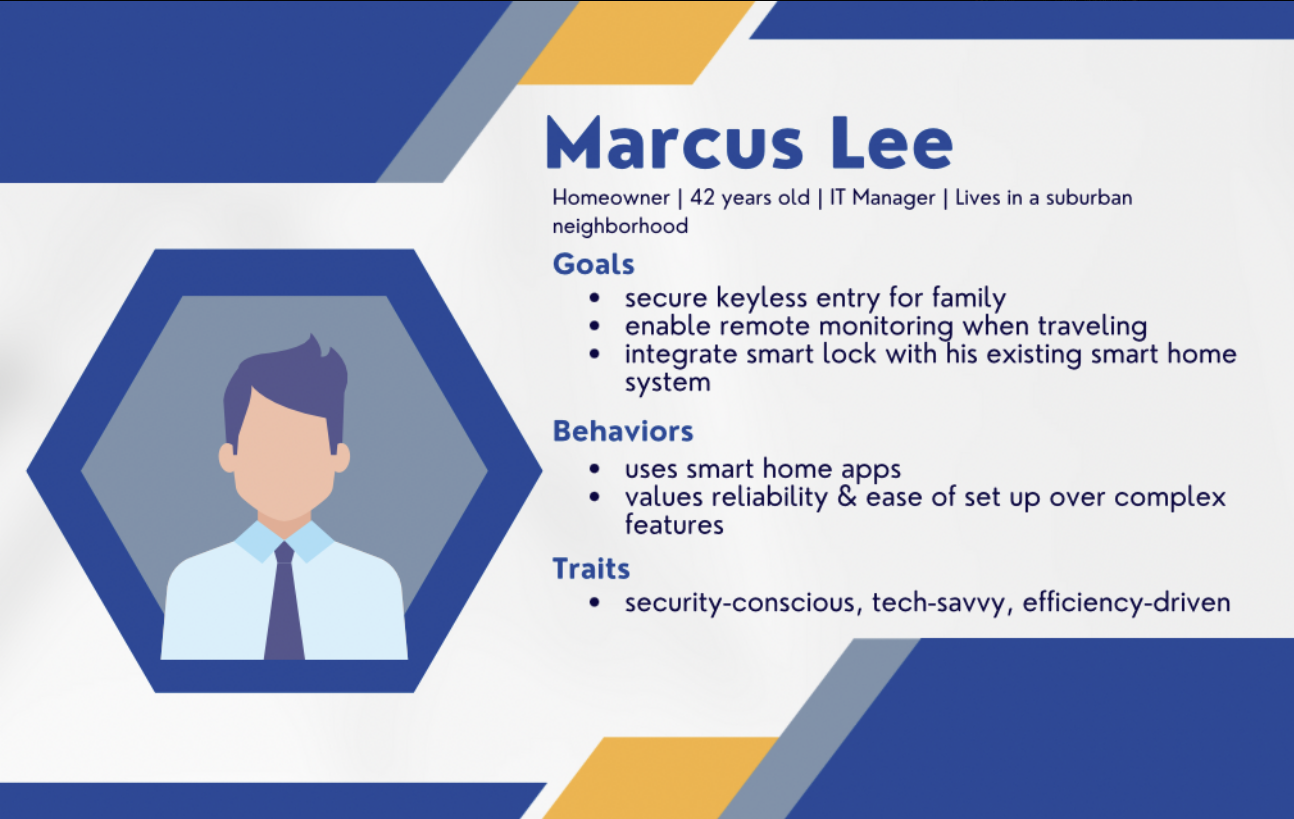
\includegraphics[width=110mm,scale=0.4]{./img/Persona1.png}
%     \label{fig:persona1}
% \end{figure}

\subsection*{Persona 2}
\begin{figure}[!ht]
    \centering
    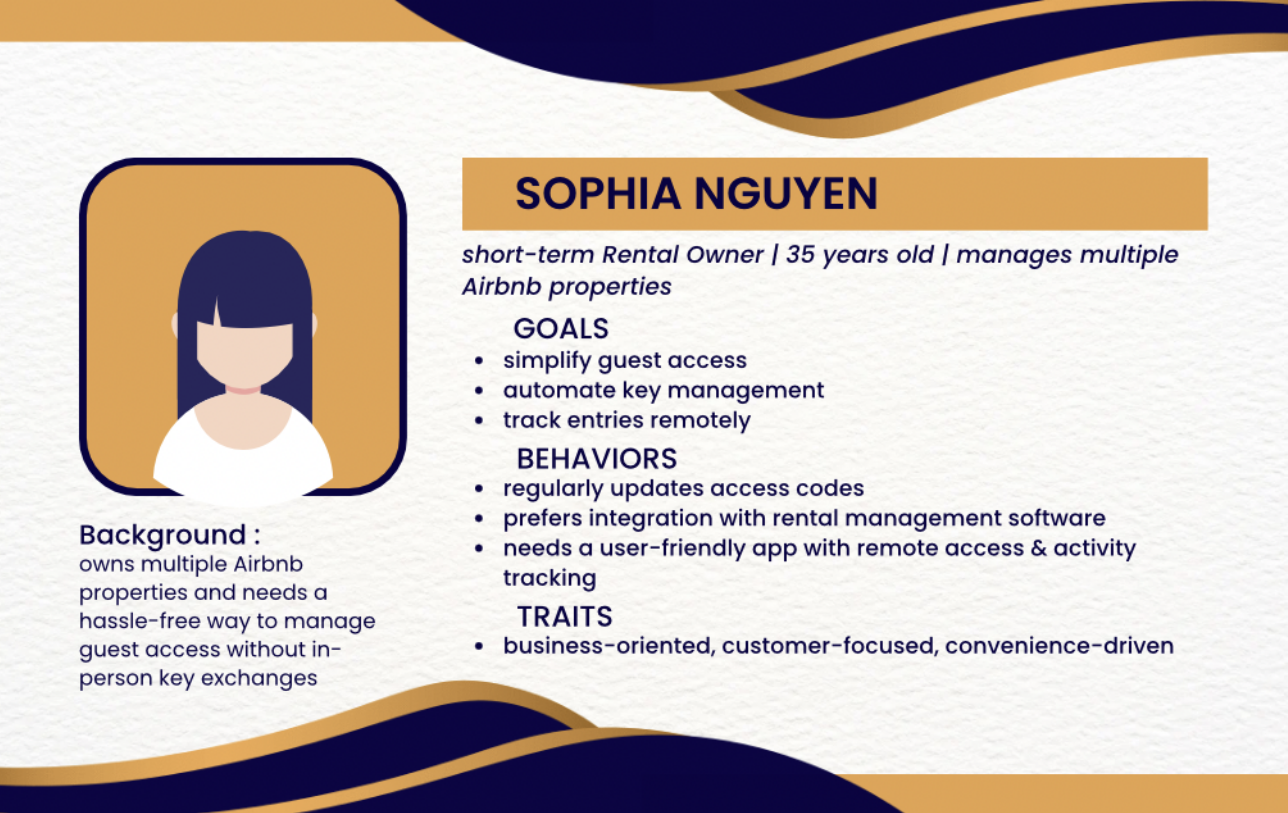
\includegraphics[width=110mm,scale=0.4]{./img/Persona2.png}
    \label{fig:persona2}
\end{figure}
\newpage


\subsection{Problem Definition}

\subsubsection{Need \& Goal Statements}
\begin{itemize}
    \item Need Statement - Traditional lock-and-key systems are inconvenient and insecure, as users may forget, lose, or have their keys stolen. Additionally, they obviously lack remote access, making it difficult for someone to enter the building if someone lost/forgot their tiny key.
    
    \item Goal Statement - Our smart lock will address these issues by enabling remote locking and unlocking, getting rid of the need for physical keys, and ensuring secure authentication for authorized users.
\end{itemize}


\subsubsection{Design Objectives}
\begin{itemize}
    \item Remote access \& control: ESP32-C3 connection with Firebase
    
    \item Local authentication via keypad:
    \item Store \& validate PINs securely using Firebase cloud
    \item Multi-user support
    \item solenoid lock integration with ESP32

\end{itemize}

\newpage
\section{Installation}

\subsection{Phone App Installation}
Open up the pamphlet included with the smart lock system. Inside, you will find a QR code labeled "App Download." Using your smartphone, scan the QR code to be redirected Google Play or Apple App Store.

Once the page loads:
\begin{enumerate}
    \item Tap \textbf{Download} or \textbf{Install}.
    \item After installation is complete, open the app.
    \item Create an account using your email and a secure password, or log in if you already have an account.
    \item Grant the necessary permissions for Bluetooth and Location if prompted.
\end{enumerate}

The app is now ready to pair with your smart lock.

\subsection{Smart Lock Installation}
Follow these steps to install the smart lock on your door:

\begin{enumerate}
    \item Remove the existing lock hardware from your door.
    \item Align the provided smart lock mounting plate with the existing holes and secure it using the included screws and screwdriver.
    \item Attach the smart lock unit onto the mounting plate. Ensure all connections are secure and the lock is properly aligned.
    \item Insert the provided batteries into the battery compartment. The device should power on automatically.
    \item Open the mobile app, go to the \textbf{Devices} section, and tap \textbf{Add New Lock}.
    \item Follow the on-screen instructions to pair the lock with your phone via Bluetooth or Wi-Fi.
    \item Once paired, test the lock by tapping the \textbf{Lock} and \textbf{Unlock} buttons within the app.
\end{enumerate}

Your smart lock is now installed and ready for use. Refer to the Troubleshooting section if you encounter any issues during setup.


\newpage
\section{Concepts Considered}

\subsection{6-3-5 Method}
\subsubsection*{Hardware \& Mechanics}
\begin{itemize}
    \item use a servo motor for deadbolt control
    \item hall effect sensor to detect if the door is open or closed
    \item implement linear actuator for silent locking
    \item maybe anti-backlash gears to reduce mechanical play
    \item consider designing a modular lock housing with 3D-printed parts
    \item have a backup battery to ensure operation during power outages
\end{itemize}

\subsubsection*{Smartphone Integration}
\begin{itemize}
    \item develop a smartphone app for remote locking/unlocking
    \item push notifications for lock activity (ex: ``Door locked at 3:45 PM'')
    \item have biometric authentication (Face ID or fingerprint)
    \item Use Bluetooth for proximity-based auto-unlock
    \item NFC support for quick unlocking via phone tap
    \item include multi-user access control with time-based permissions
\end{itemize}

\subsubsection*{Security Features}
\begin{itemize}
    \item Implement AES-256 encryption for communication between the lock and phone
    \item maybe two-factor authentication for app access
    \item develop a tamper-detection alarm if the lock is forced
    \item lockdown mode for multiple failed attempts
    \item include a manual override mechanism in case of system failure
    \item utilize rolling codes for Bluetooth pairing to prevent hacking
\end{itemize}

\subsubsection*{Software \& Control}
\begin{itemize}
    \item ESP32 microcontroller for Wi-Fi and Bluetooth control
    \item Develop a closed-loop system to verify if the lock is engaged properly
    \item make a real-time event log accessible via the app
    \item add a scheduling feature for auto-locking at specific times
    \item guest mode with temporary passcodes
    \item Integration with voice assistants like Alexa or Google Assistant
\end{itemize}

\subsubsection*{Advanced Features}
\begin{itemize}
    \item GPS stuff
    \item add geofencing to lock or unlock based on the user's location
    \item integrate with smart home platforms like Home Assistant
    \item use AI-based behavior analysis to suggest locking patterns
    \item add a camera with facial recognition for auto-unlock
    \item enable remote firmware updates
    \item learn database SQL
    \item use solar charging for battery-powered locks
\end{itemize}



% BRAINSTORMING -----------------------------




\subsection{Brainstorming}

\subsubsection*{Adam Wu}
\begin{itemize}
    \item As a person who has amnesia, I would like to be able to find my keys anytime so that when I forget where I place them, I can find them.
    \begin{itemize}
        \item Having a "find my" solution with a key.
    \end{itemize}
    \item As a person who loves security, I would like to have the best lock for my house so that lock pickers are not able to pick my lock.
    \begin{itemize}
        \item Making an “authentication” key that resets the key code within a set time, making it harder for hackers to unlock the door.
    \end{itemize}
    \item As a person who is always last-minute out the door, I fear forgetting to lock the door when I close it.
    \begin{itemize}
        \item Auto-locking door when a person closes the door.
    \end{itemize}
    \item As a person who often forgets to bring their keys, I am scared of getting locked out.
    \begin{itemize}
        \item Having a notification from the key to the phone that alerts: “keys are not close by to you.”
    \end{itemize}
    \item As a parent, I am scared of my kids forgetting their keys and locking themselves out of their room.
    \begin{itemize}
        \item Creating a “master key” that only parents/admins can use to unlock specific doors.
    \end{itemize}
    \item Concerned about key battery life.
    \begin{itemize}
        \item Send a notification to the user when the key is on low battery.
    \end{itemize}
\end{itemize}

\subsubsection*{Nathaniel Laurente}
\begin{itemize}
    \item Key has the ability to notify the user when too far away from the user’s phone/body.
    \item Key deactivates/won’t be able to open the door if too far away from the owner.
    \item “Tap to Pay” technology concept.
    \begin{itemize}
        \item Unlocks the door like a credit card tap on a phone.
        \item If too complex, explore alternative ways to unlock the door.
        \item Eliminates the need for a physical key.
        \item Prevents stolen keys from working if the user still has their phone.
    \end{itemize}
    \item Secure deactivation of the key when too far from the user.
    \begin{itemize}
        \item Possible solution: Use the user's phone for deactivation.
    \end{itemize}
    \item One-time password generator between lock and key to ensure only this exact key can enter the house.
    \item Backup way to get into the house if the user forgets/loses their key.
    \begin{itemize}
        \item Pin access code.
        \item App allows for 2FA authentication using a thumbprint and/or Face ID.
    \end{itemize}
    \item Will the battery last long enough for multiple years?
\end{itemize}

\subsubsection*{Neena Nguyen}
\begin{itemize}
    \item Existing smart lock solutions:
    \begin{itemize}
        \item Smart locks for dorm rooms using mobile apps, passcodes, and scanners.
    \end{itemize}
    \item Who will use this lock?
    \begin{itemize}
        \item People with memory issues (elderly, ADHD).
        \item University students in dorm rooms.
        \item Student ID scanner integration.
        \item Parents with small children (child-proof locks).
    \end{itemize}
    \item Features for parental control.
    \begin{itemize}
        \item Locks after a curfew time.
        \item Prevents children from unlocking without parental approval.
        \item Alerts parents when kids come home from school.
    \end{itemize}
    \item What kind of door lock will it be?
    \begin{itemize}
        \item Facial recognition (requires camera and database knowledge).
        \item Logs entry and exit timestamps.
        \item Digital passcode through an app.
        \item Auto-relocking mechanism after failed attempts.
        \item Bluetooth detection for unlocking within a certain range.
        \item Dual authentication (PIN + scan).
        \item Optional security trigger after specific hours.
        \item Alerts when the door is left unlocked for too long.
        \item Auto-locking after prolonged unlocking.
        \item Detection system to check if the key is on the person.
        \item Prevents intruders from entering without a key.
    \end{itemize}
\end{itemize}

\subsubsection*{Jackson Kennedy}
\begin{itemize}
    \item Normal keys can be lock-picked, but digital keys can be secured based on a communication protocol.
    \item Secure authentication methods.
    \begin{itemize}
        \item PIN authentication with 2FA.
        \item Optimal PIN length (e.g., 4-digit PIN has 1,048,576 combinations).
        \item Brute force prevention strategies.
    \end{itemize}
    \item Preventing communication protocol vulnerabilities.
    \begin{itemize}
        \item What protocol should be used? (Bluetooth has vulnerabilities and short range.)
        \item Cloud-based solutions rely on third-party vendor security.
        \item What information needs to be transferred? (Video data, authentication signals?)
    \end{itemize}
    \item Lock activation logic.
    \begin{itemize}
        \item How exactly will the lock know when to unlock? (Sending a 0 or 1 signal based on specific conditions?)
    \end{itemize}
    \item Security and alerting technologies.
    \begin{itemize}
        \item Sensors to detect nearby people.
        \item Hidden camera or biometric verification for identity confirmation.
    \end{itemize}
    \item Scheduling and timed access.
    \begin{itemize}
        \item Physical locks do not have scheduling options.
        \item Implement timed unlocking (e.g., unlock for 15 minutes for a babysitter).
        \item Extra verification to prevent intruders from exploiting schedules.
    \end{itemize}
\end{itemize}
\newpage









% Begin Morphological Charts ----------------------------------

\subsection{Morphological Charts}

\begin{figure}[!ht]
    \centering
    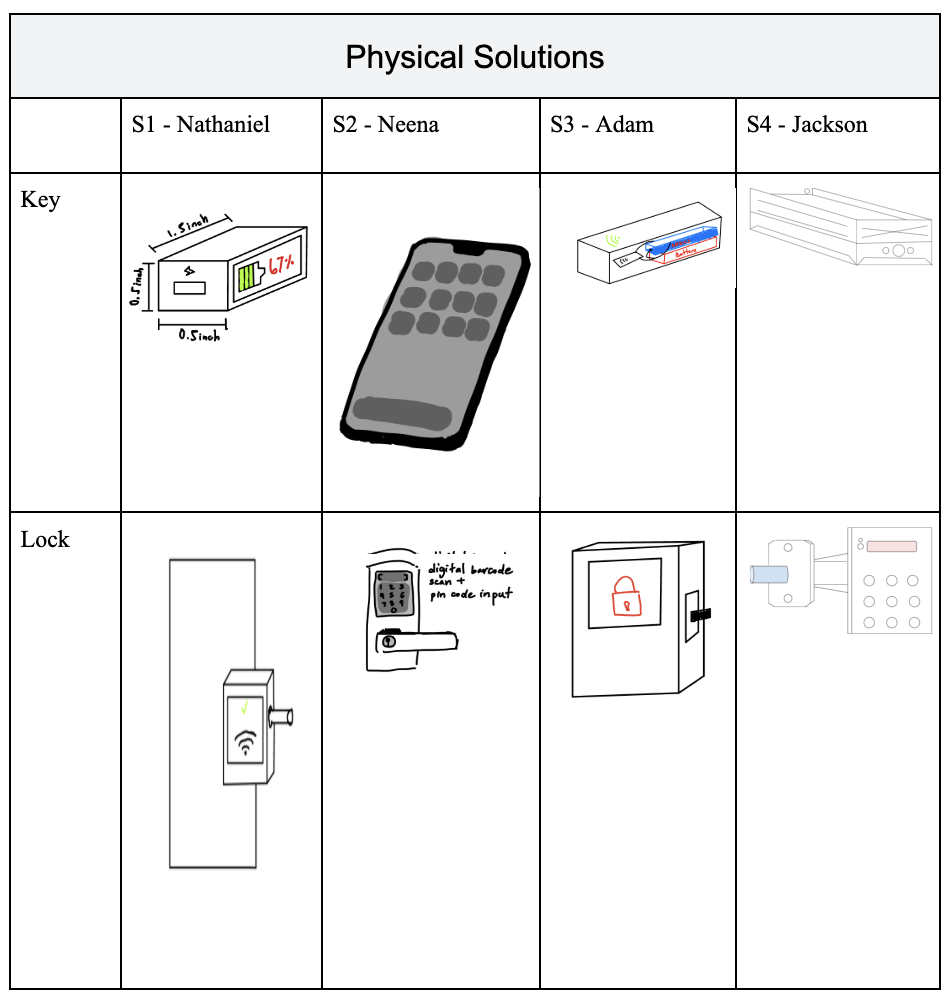
\includegraphics[width=1\linewidth]{./img/p1mm.png}
    \caption{Physical Solution Chart}
    \label{fig:p1mm}
\end{figure}
\newpage
\begin{figure}[!ht]
    \centering
    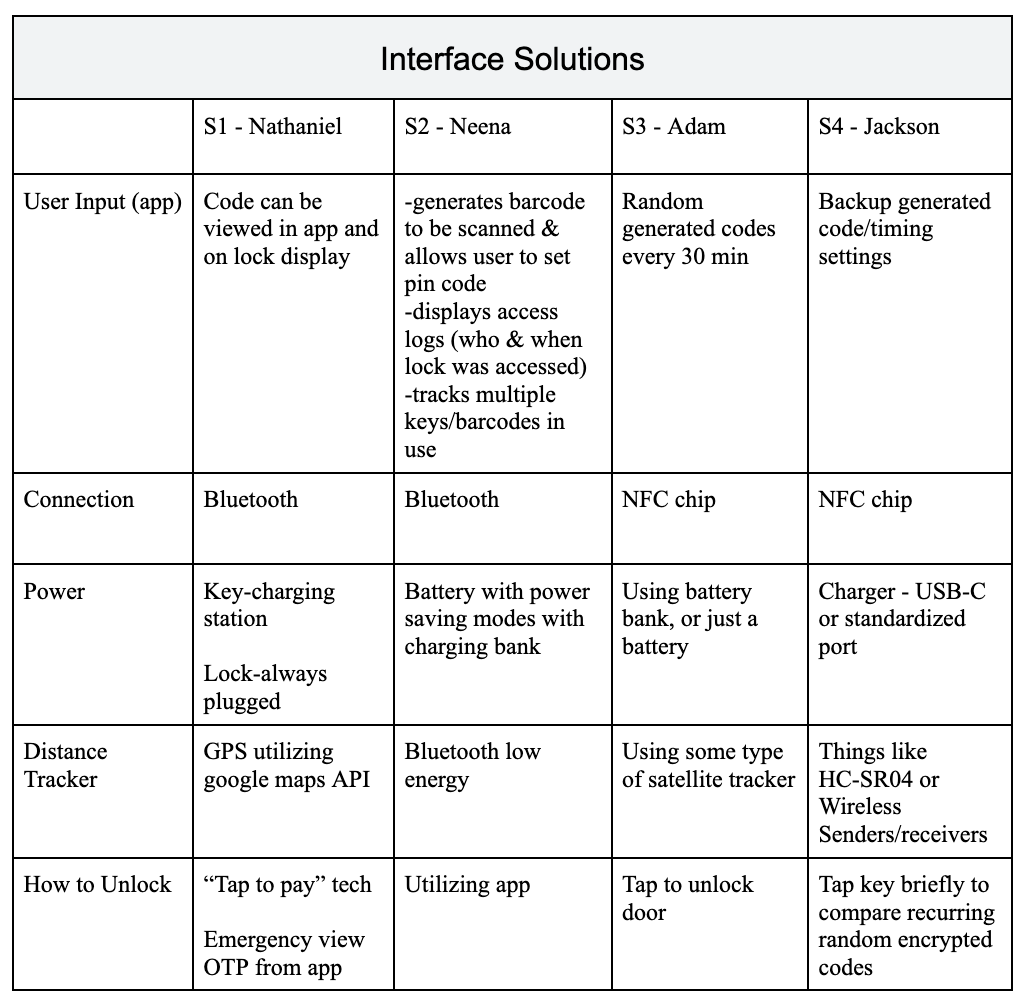
\includegraphics[width=1\linewidth]{./img/p2mm.png}
    \caption{Interface Solutions}
    \label{fig:p2mm}
\end{figure}
\newpage





% Begin Mind Map ---------------------------------------------

\subsection{Mind Map}

\begin{figure}[!ht]
    \centering
    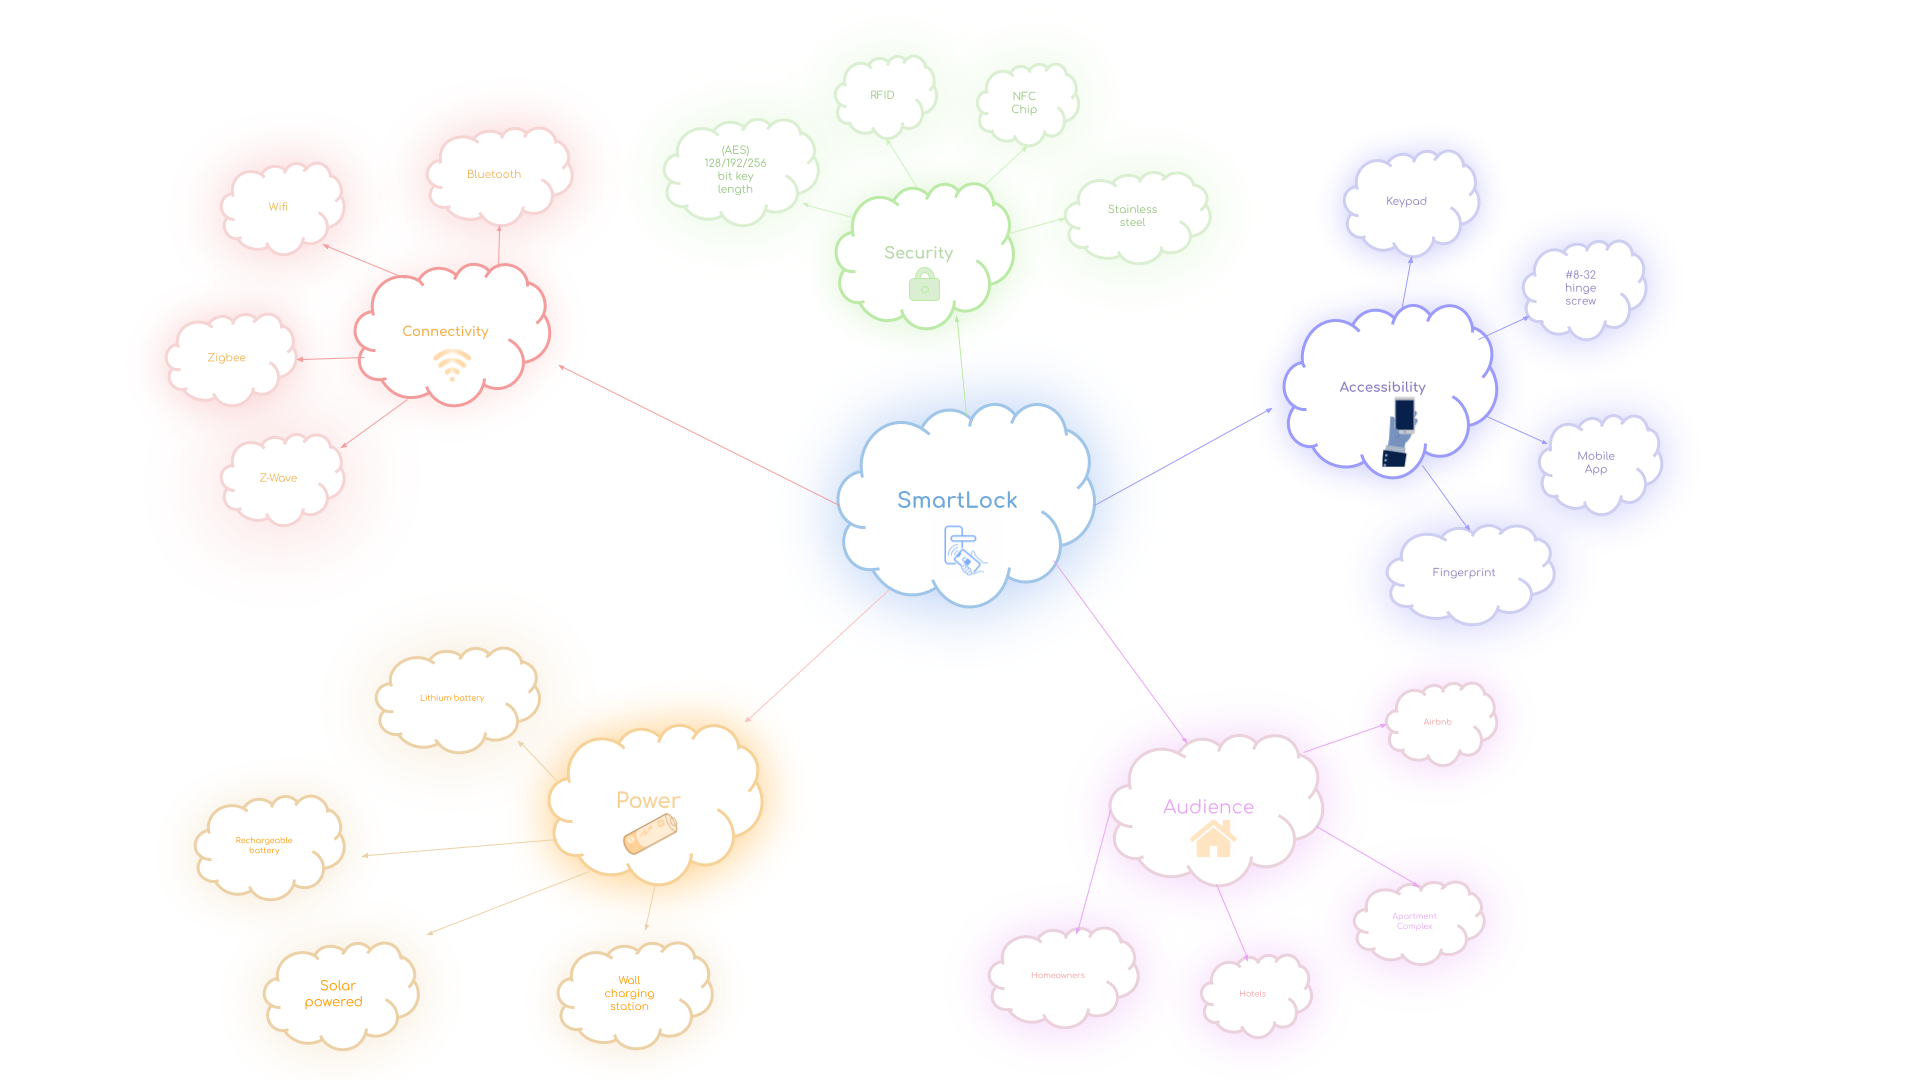
\includegraphics[width=140mm,scale=0.5]{./img/mindmapsmartlock.png}
    \caption{Mind Map}
    \label{fig:mindmapsmartlock}
\end{figure}
\newpage

\subsection{Concept Selection}

\subsubsection{Weighting Factors}
\begin{tabular}{ll}
    \toprule
    Criteria & Weight (\%) \\
    \midrule
    Security & 40 \\
    Cost & 30 \\
    Power Consumption & 20 \\
    User Convenience & 10 \\
    \textbf{Total} & \textbf{100} \\
    \bottomrule
\end{tabular}

\subsubsection{Decision Table}
\resizebox{\textwidth}{!}{%
\begin{tabular}{lcccc}
    \toprule
    Criteria & Weight & Design 1 (Basic) & Design 2 (Mid-Range) & Design 3 (Advanced) \\
    \midrule
    Security & 40 & 6 (240) & 8 (320) & 10 (400) \\
    Cost & 30 & 10 (250) & 6 (150) & 3 (75) \\
    Power Consumption & 20 & 6 (90) & 8 (120) & 10 (150) \\
    User Convenience & 10 & 3 (30) & 6 (60) & 9 (90) \\
    \textbf{Total Score} & \textbf{100} & \textbf{680} & \textbf{720} & \textbf{780} \\
    \bottomrule
\end{tabular}%
}

\textbf{Best Design:} Design 3 (Advanced) with 780 points, prioritizing security, cost-efficiency, and power optimization.

\newpage


% Actual Design of Marketable Product
\newpage
\subsection{Transitioning SmartLock from Prototype to Market-Ready Product}

To move from a functional prototype to a marketable SmartLock product, several key engineering and business steps need to be addressed. This involves refining both hardware and software components, ensuring scalability and security standards.

\subsubsection{Custom Hardware Design}

The ESP32 microcontroller used in the prototype provides an platform for development and proposal, but a custom-designed microcontroller will offer improved performance, cost-efficiency, power-efficiency, and security.

\begin{itemize}
  \item \textbf{PCB Design:} Develop a custom printed circuit board (PCB) integrating a microcontroller with essential peripherals (e.g., motor drivers, Wi-Fi/Bluetooth module, battery management).
  \item \textbf{Power Optimization:} Ensure low-power operation modes and efficient battery usage for real-world longevity.
  \item \textbf{Form Factor:} Design a compact form to fit lock, pin-pad, microcontroller dimensions and installation constraints.
  \item \textbf{Manufacturability:} Optimize for scalable manufacturing, component sourcing, manufacture, and assembly.
\end{itemize}

\subsubsection{Backend Infrastructure Development}

Firestore offers an accurate prototype, but a production system needs more control, security, and scalability.

\begin{itemize}
  \item \textbf{Cloud-Based Database:} Develop a backend using platforms such as AWS, Azure solution with REST/GraphQL APIs.
  \item \textbf{Security Architecture:} Implement end-to-end encryption, secure authentication, and role-based access control.
  \item \textbf{Real-Time Communication:} Use MQTT or WebSockets for real-time lock state updates.
\end{itemize}

\subsubsection{Mobile/Web App Enhancement}

The current web interface can be transformed into a polished, user-friendly app for mainstream adoption.

\begin{itemize}
  \item \textbf{Cross-Platform Support:} Build using Flutter, React Native, or Swift/Kotlin for Android and iOS platforms.
  \item \textbf{User Experience (UX):} Incorporate intuitive design, user onboarding, remote lock/unlock, and notification features.
\end{itemize}

\subsubsection{Compliance and Security Certification}

A production-ready smartlock must comply with legal standards and certifications.

\begin{itemize}
  \item \textbf{Certifications:} Obtain CE, FCC, or other regional certifications for wireless and electronic devices.
  \item \textbf{Privacy Compliance:} Ensure GDPR/CCPA compliance with respect to user data handling and storage.
\end{itemize}




% Design of Manufacture addition
\subsection{\textcolor{gray}{Detail of Design}}
The Smart Lock prototype consists of both hardware and software components, designed to provide secure, remote access control with user authentication and cloud connectivity.

\subsubsection{\textcolor{teal}{System Overview}}

Our system integrates a physical keypad-based lock with Wi-Fi-enabled remote access through a mobile application. Users can authenticate using a PIN or biometric authentication (fingerprint or facial recognition), and manage access remotely.

\begin{figure}[h]
    \centering
    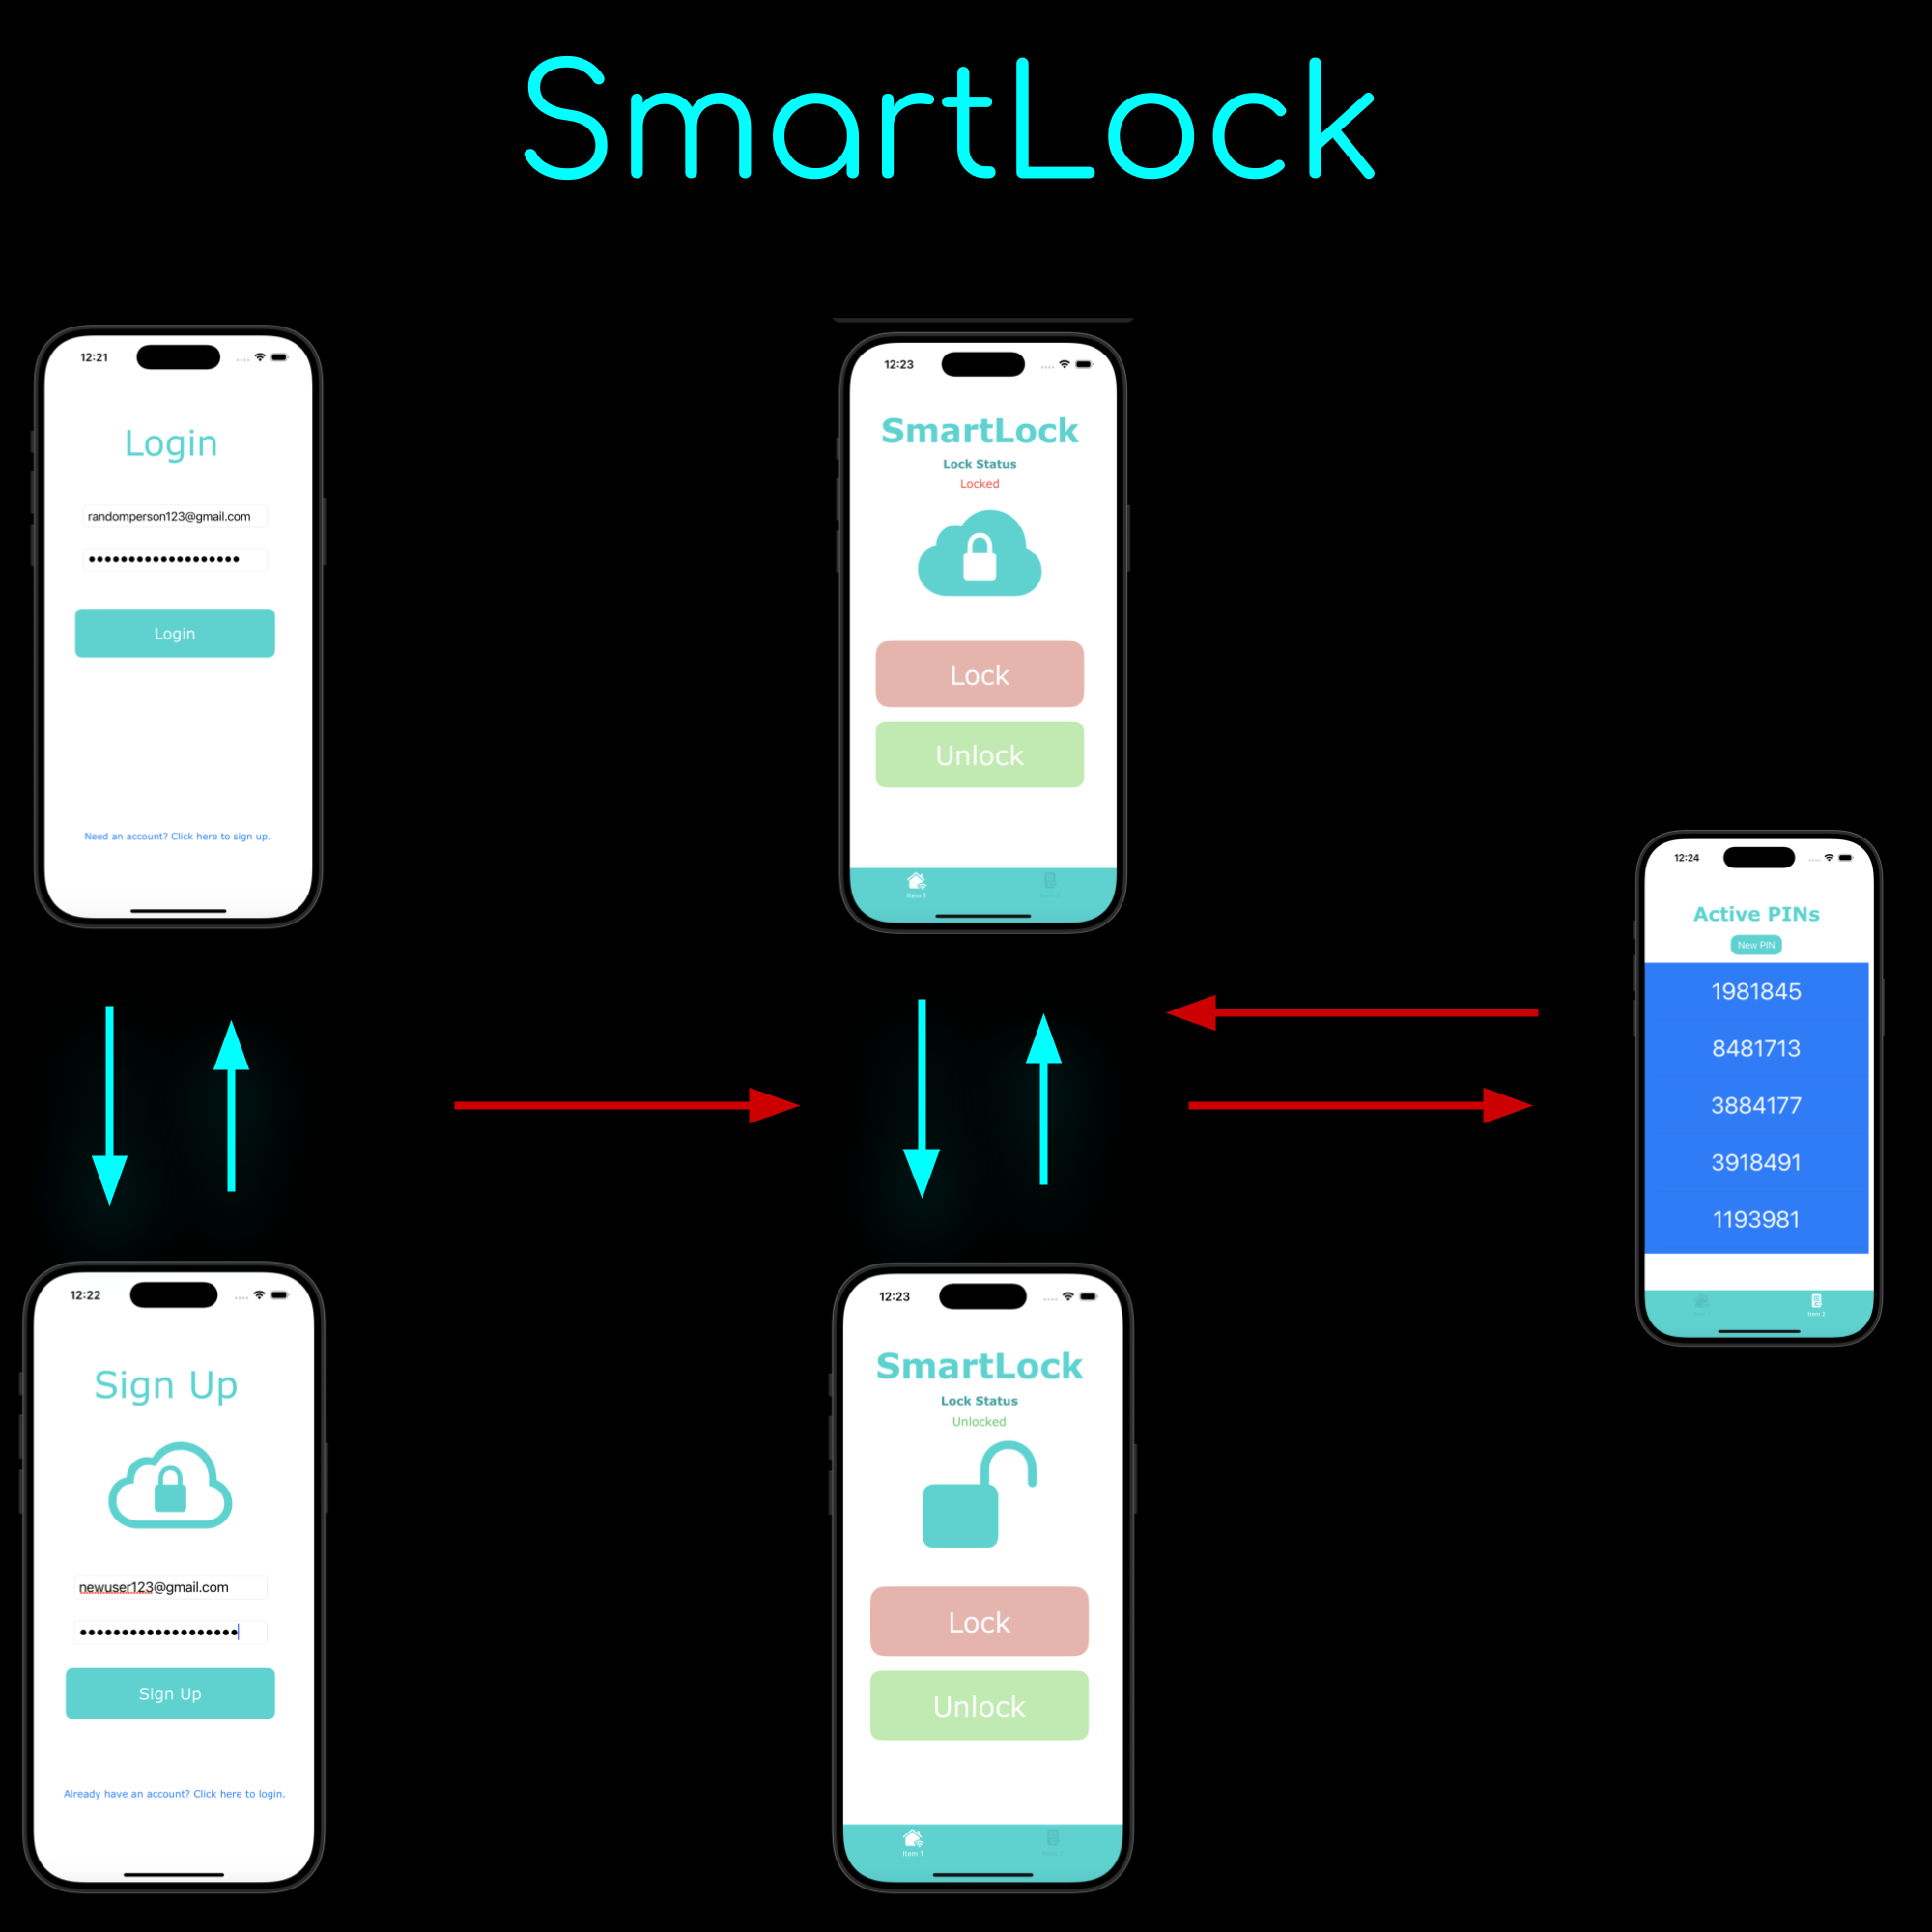
\includegraphics[width=0.65\textwidth]{flowsl.png}
    \caption{Mobile App Flowchart for Smart Lock System}
\end{figure}

\begin{itemize}
    \item Users log in or create an account to access the smart lock.
    \item The main control screen provides lock/unlock buttons.
    \item Users can view and manage active PIN codes for secure access.
    \item The system communicates with a cloud database (Firestore) for real-time authentication and remote control.
\end{itemize}

\subsubsection{\textcolor{teal}{Connectivity and Cloud Integration}}

The Smart Lock is cloud-connected, enabling users to manage access remotely via a mobile app. The system:
\begin{itemize}
    \item Authenticates PIN entries locally for quick access.
    \item Processes biometric authentication for increased security.
    \item Syncs PIN codes with Firebase, allowing updates in real-time.
    \item Sends lock/unlock status to the cloud, ensuring remote monitoring.
    \item Logs user access, creating an audit trail for security.
\end{itemize}

\subsubsection{\textcolor{teal}{Hardware Design}}

The Smart Lock hardware consists of a 3D printed casing, a keypad for PIN entry, a biometric scanner, a solenoid lock mechanism, and an ESP32-C3 microcontroller.

\begin{figure}[htbp]
    \centering
    \begin{subfigure}[b]{0.48\textwidth}
        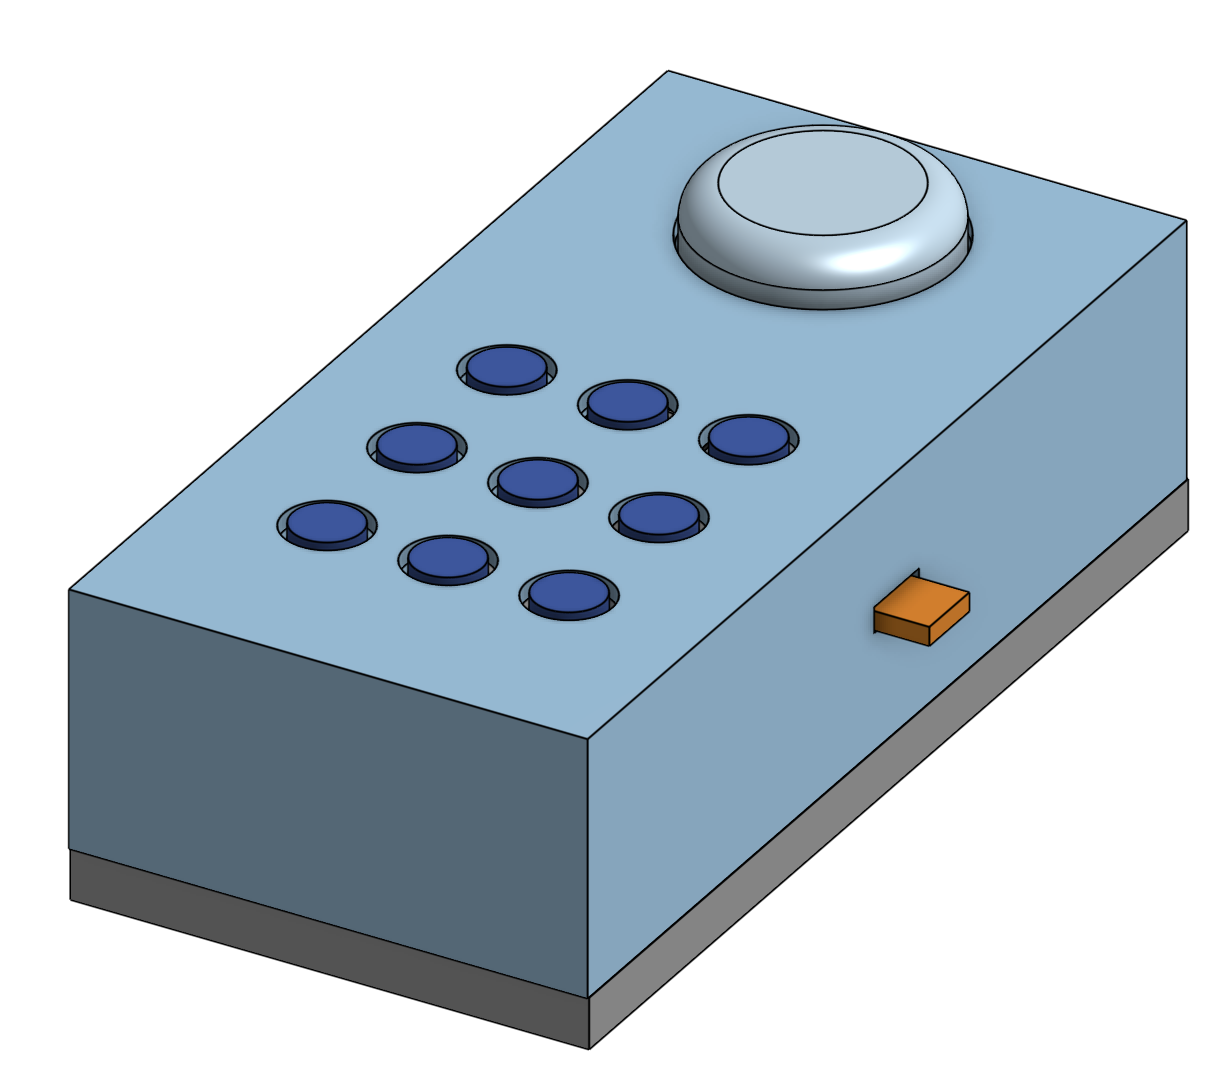
\includegraphics[width=\textwidth]{./isoView.png}
        \caption{Isometric View}
        \label{fig:isoView}
    \end{subfigure}
    \hfill
    \begin{subfigure}[b]{0.48\textwidth}
        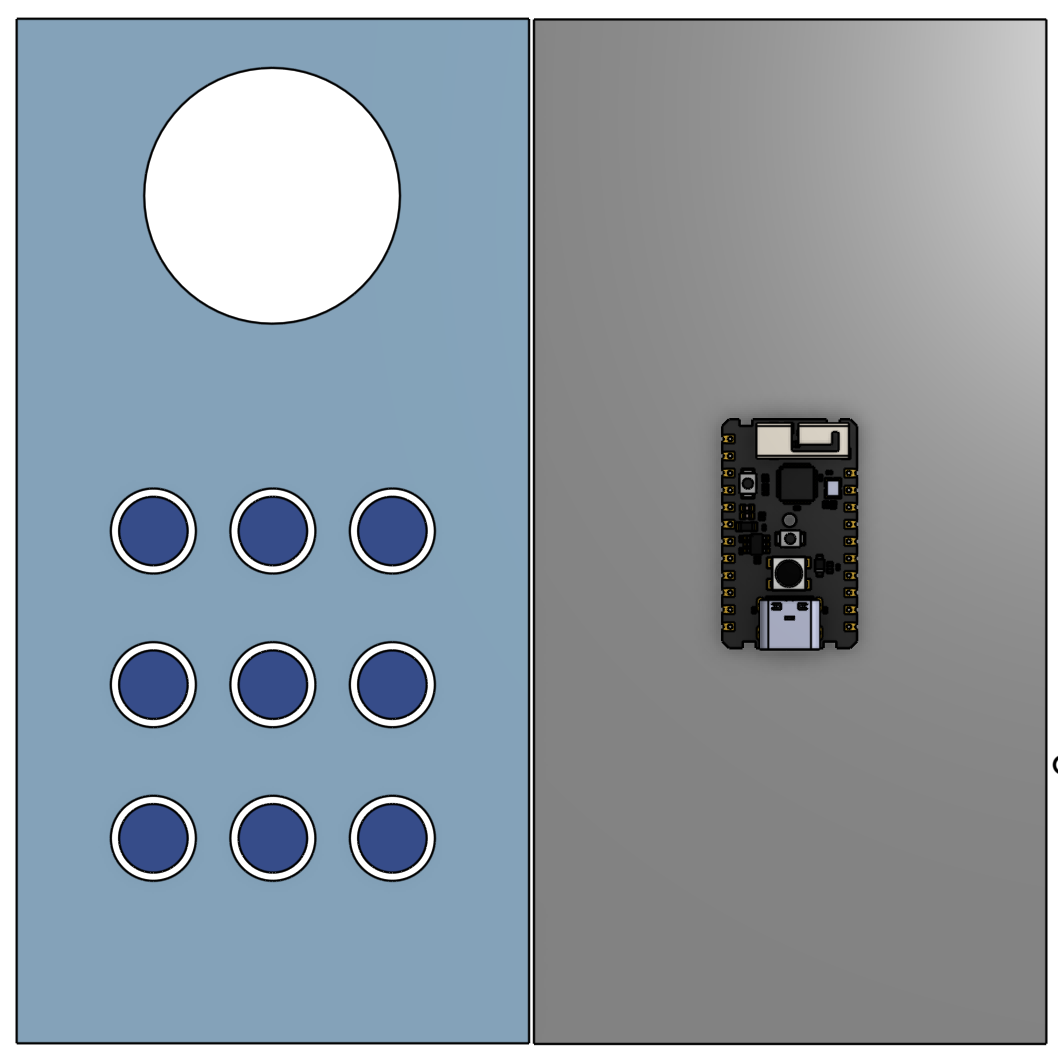
\includegraphics[width=\textwidth]{./topView.png}
        \caption{Top View}
        \label{fig:topView}
    \end{subfigure}
    \caption{First lock design}
\end{figure}

Here is the isometric view of the Smart Lock prototype. The top section will potentially include a biometric scanner, for fingerprint or facial recognition authentication, and a numeric keypad for PIN entry.\newline

\textbf{Key components:}
\begin{itemize}
    \item \textbf{Biometric Scanner:} Supports fingerprint or facial recognition for enhanced security
    \item \textbf{Numeric Keypad:} Users enter PIN codes as an alternative authentication method
    \item \textbf{Solenoid Lock:} Engages or disengages upon successful authentication
    \item \textbf{Microcontroller (ESP32-C3):} Handles user input, authentication, and connectivity
    \item \textbf{Rechargeable Battery:} Powers the system, ensuring reliability even in case of power outages
\end{itemize}

This design ensures compactness while maintaining modular repairability, allowing components to be easily accessed or replaced.


\subsubsection{\textcolor{teal}{Life Cycle Assessment (LCA)}}

The life cycle of the Smart Lock was analyzed to ensure sustainability and environmental responsibility. Key aspects include: \newline

\textbf{Eco-Friendly Manufacturing}
\begin{itemize}
    \item Uses locally sourced materials to minimize transportation emissions
    \item Modular design allows for easy repair and component replacement, reducing e-waste
    \item Prioritizes recyclable materials in construction
\end{itemize}

\textbf{Energy Efficiency}
\begin{itemize}
    \item Operates on a rechargeable lithium battery to extend lifespan
    \item Supports an optional solar charging module to reduce reliance on disposable batteries
\end{itemize}

% Battery Life and Design
\newpage
\subsection{Battery Power Management and Notification System}

While the prototype operates on a continuous power source, a commercial SmartLock will use a secure, long-lasting battery to ensure usability during power outages and in locations without fixed power. Proper battery management involves monitoring charge levels, notifying users, and providing a safe and secure method for recharging or replacing the battery.

\subsubsection{Battery Selection and Power Optimization}

Selecting the right battery type and minimizing power consumption are critical for long-term operation.

\begin{itemize}
  \item \textbf{Battery Type:} Use high-capacity rechargeable lithium-ion or lithium-polymer batteries capable of lasting several months on a single charge.
  \item \textbf{Low Power Modes:} Implement deep sleep and wake-on-interrupt features in the firmware to minimize power draw during idle periods.
\end{itemize}

\subsubsection{Battery Monitoring and User Notification}

Monitoring battery status and notifying users to ensure maintenance and avoid unexpected lockouts.

\begin{itemize}
  \item \textbf{Voltage Monitoring Circuit:} Integrate a voltage divider or dedicated battery management gauge to continuously monitor battery levels.
  \item \textbf{Battery State Logging:} Periodically upload battery status to the cloud alongside status logs.
  \item \textbf{User Notifications:} Send low battery alerts via push notifications, email, or in-app messages when battery drops below a critical threshold (e.g., 30\%).
\end{itemize}

\subsubsection{Safe and Secure Battery Replacement or Recharging}

Users must be able to service the battery safely without compromising lock security or usability.

\begin{itemize}
  \item \textbf{Secure Battery Access:} Design an internal battery compartment accessible only when the lock is in an unlocked state or with a secure override mechanism.
  \item \textbf{Rechargeable Design:} Provide a USB-C or magnetic charging port for easy recharging without disassembling the lock.
  \item \textbf{Tamper Detection:} Include log entries if the battery compartment is accessed, and notify the owner.
  \item \textbf{Backup Power Support:} Consider integrating a backup battery to retain state data during battery swap, or integrate a way to reset lock data upon battery replacement or recharge.
\end{itemize}


% Ownership/Access Control + History and Status Logging
\subsection{Ownership and Access Control}

Managing ownership and granting user access are critical to ensuring that SmartLock devices remain secure while allowing for flexible sharing. This system must allow primary users to delegate lock access to other users, while ensuring that the delegated users have the appropriate permissions.

\subsubsection{Ownership Model}

Each SmartLock must have a primary owner who holds full control over the device and its permissions.

\begin{itemize}
  \item \textbf{Lock Registration:} When a new lock is initialized, the registering user becomes the owner.
  \item \textbf{Ownership Table:} Store ownership information in the database alongside lock records (e.g., \texttt{lock\_id}, \texttt{owner\_id}).
\end{itemize}

\subsubsection{Access Delegation and Permissions}

Primary owners can grant access to other users, allowing them to interact with specific locks under defined conditions.

\begin{itemize}
  \item \textbf{Access Table:} Maintain a table or collection with fields such as \texttt{lock\_id}, \texttt{user\_id}, \texttt{access\_level} (view, control), \texttt{granted\_by}, and \texttt{expiration} if necessary.
  \item \textbf{Access Rights Enforcement:} Backend logic and security rules should enforce permissions before allowing user actions.
  \item \textbf{Revocation and Expiration:} Include features for the owner to revoke access at any time or set expiration timers for temporary access.
\end{itemize}

\subsubsection{User Interface for Access Management}

The frontend application should allow users to manage and review access settings.

\begin{itemize}
  \item \textbf{Access Dashboard:} Display which users currently have access to a given lock and their permission levels.
  \item \textbf{Invite Flow:} Enable owners to invite users via email or user ID, specifying which lock(s) they can access.
\end{itemize}

%%%%%%%%%%%%%%%%%%%%%%%%%
%
%
% History and Logging
%
%
%%%%%%%%%%%%%%%%%%%%%%%%%

\newpage
\subsection{History and Status Logging}

 Logging improves security, aids in diagnostics, and enhances transparency for users. The SmartLock system should log both user actions and technical status changes.

\subsubsection{History Log of User Actions}

Tracking user interactions with locks helps in audits, diagnostics, and usage insights.

\begin{itemize}
  \item \textbf{Log Entry Fields:} Include \texttt{timestamp}, \texttt{user\_id}, \texttt{lock\_id}, and \texttt{action} (e.g., lock, unlock, access granted).
  \item \textbf{Database:} Automatically write to the history log whenever a user successfully executes an action.
  \item \textbf{User Access to Logs:} Allow users to view logs for locks they own or have access to.
\end{itemize}

\subsubsection{Status Log for Lock Health Monitoring}

Status logs are essential for monitoring device reliability and connectivity.

\begin{itemize}
  \item \textbf{Microcontroller Event Logging:} Program the microcontroller to push logs to Cloud structure or a backend data on significant events (e.g., Wi-Fi reconnect, battery low).
  \item \textbf{Technical Dashboard:} Visualize connection stability and firmware state for each lock.
\end{itemize}

\subsubsection{Action Confirmation and Notifications}

Users must be notified when actions are completed to reinforce trust and responsiveness.

\begin{itemize}
  \item \textbf{Action Acknowledgement:} ESP32 should confirm action execution back to Cloud database (e.g., “locked: true”).
  \item \textbf{Notification Service:} Use real-time updates to the mobile app or web interface.
  \item \textbf{Failure Alerts:} Alert users if an action fails, with details such as connectivity issues or mechanical faults.
\end{itemize}


% Installation Process after receiving the product
\newpage
\subsection{Initial Installation and Setup Procedure}

The following outlines the essential steps required to ensure a seamless setup and onboarding experience for end users upon receiving the SmartLock. This section is intended to guide engineers in implementing a standardized process that balances user-friendliness with robust technical integration. The procedure includes steps from unboxing to successful WiFi provisioning via Bluetooth communication.

\subsubsection{Step 1: Unboxing and Physical Inspection}

Upon receipt of the SmartLock device, users are expected to perform a basic inspection of the package contents.

\begin{itemize}
    \item Ensure all components are present:
        \begin{itemize}
            \item SmartLock main unit
            \item Mounting bracket and screws
            \item Quick-start guide with QR Code at Front Page (printed)
        \end{itemize}
    \item Verify the unit is free of visible defects or damage.
    \item Charge the unit if not pre-charged (optional: LED will indicate low battery if charging is required).
\end{itemize}

\subsubsection{Step 2: Mobile Application Download}

Before any configuration can begin, users must download the official SmartLock companion app. The app serves as the bridge between the mobile device and the lock, handling both Bluetooth communication and network provisioning.

\begin{itemize}
    \item Available on iOS (App Store) and Android (Google Play Store).
    \item App name: \textbf{SmartLock Home}.
    \item Version requirement: iOS 13+ / Android 9+.
    \item Upon opening the app, users must grant Bluetooth and location permissions as required by the mobile OS.
\end{itemize}

\subsubsection{Step 3: Initial Bluetooth Pairing}

Once the app is installed, users are prompted to begin the pairing process via Bluetooth. This enables the mobile device to establish a secure connection with the SmartLock unit.

\begin{itemize}
    \item The SmartLock should be placed in pairing mode. This is triggered automatically on first boot, indicated by a flashing blue LED.
    \item The app will scan for nearby devices. The SmartLock will be listed as \texttt{SmartLock-XXXX}, where \texttt{XXXX} represents the last 4 digits of the device's MAC address.
    \item Once selected, the user will initiate pairing. This may include a confirmation prompt or PIN verification depending on device configuration.
    \item A secure Bluetooth connection will be established upon successful pairing.
\end{itemize}

\subsubsection{Step 4: WiFi Provisioning}

After a secure Bluetooth channel has been established, the next phase involves transferring the user's WiFi credentials to the SmartLock for permanent network connectivity.

\begin{itemize}
    \item The mobile app will prompt the user to select a 2.4GHz WiFi network (5GHz bands are not supported).
    \item Users will enter the SSID and password of their home network.
    \item Credentials are encrypted and transmitted to the SmartLock via Bluetooth.
    \item The SmartLock attempts to connect to the provided network. Connection success or failure will be relayed to the app.
    \item Upon successful connection, the LED will turn solid green, and the app will confirm that setup is complete.
\end{itemize}

\subsubsection{Final Notes and Engineer Considerations}

\begin{itemize}
    \item Ensure Bluetooth Low Energy (BLE) is used for communication to optimize power efficiency.
    \item All user-facing steps should include error handling and clear guidance for troubleshooting.
    \item Logs of pairing attempts, WiFi status, and user interactions should be stored locally for support diagnostics.
    \item Future firmware should support Over-the-Air (OTA) updates to streamline enhancements and bug fixes.
\end{itemize}

This setup process is designed to offer an intuitive user experience while providing the flexibility and security required for a modern smart home device. Engineers should maintain this structure while accounting for evolving mobile OS standards and networking best practices.


\newpage % new section, new page
\section{Functional Prototype}

% Should talk about the hardware, software, and cloud infrastructure we used compared to what we wanted.

\subsection{Hardware}

For our functional prototype, we used the ESP32-C3 microcontroller, solenoid lock, LEDs, transistors, and a keypad. The ESP32-C3 is the brain of the entire lock, being able to send and recieve signals from the server. Compared to our manufactured design, we will be building our own microcontroller so that it is customized to have the required functionality we need for our lock. As for the solenoid lock, we also plan to use an industry standard lock so that it can actually work on a standard door. Our microcontroller reads and write to the server, then controls the door lock to either lock or unlock. Furthermore, when it finishes doing a task of locking or unlocking, it will send back an acknowledgement that the task is officially done. The microcontroller for our prototype uses wifi provisioning (acts as an access point) to let users fill in parameters of their wifi SSID and password, along side the API key. In our manufactured design though, we plan to use bluetooth to do all the setup instead of using wifi provisioning.

\subsection{Software}

The functional prototype of the app currently uses the Swift language. This is what we wanted especially for native IOS apps, and in our manufactured design we plan to use the same language. Though we also would like to produce the same app on other non IOS devices as well. The app currently is able to allow users to sign in and sign up, unlock and lock the door, generating one time pins, accessing emergency pins, and logging out. 

\subsection{Cloud infrastructure}

Our current cloud infrastructure uses firestore database from firebase. Firebase was the easiest to use for our prototyping, and allowed us to quickly made the project functional. Though for the production system, we plan to use Amazon Web Services (AWS) along side Postgres so that we have more control on our database.  The current structure of our database only have a user controlling a lock, while we plan to update our cloud structure to have a many-to-many relationship. It should have a table for users and another table for locks, this way we can create a join table to join which users owns which lock and the lock is also able to know who the owner is. This is the common way people use the cloud structure to solve the many-to-many relationship.

 % new section
% Describes what we have done compared to the manufactured design


% Begin Morphological Charts ----------------------------------

\section{Economic Analysis}
Below we have the images for DFM, DFA, and Life Cycle Assessment.
\newpage
\subsection*{DFM \& DFA}
\begin{figure}[!ht]
    \centering
    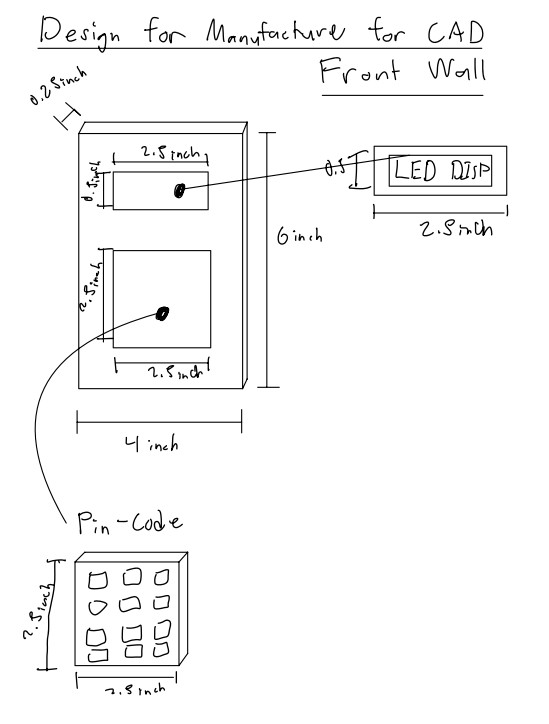
\includegraphics[width=0.8\linewidth]{img/DFM_Front_wall.png}
    % \caption{Physical Solution Chart}
    \label{fig:enter-label}
\end{figure}
\newpage

\begin{figure}[!ht]
    \centering
    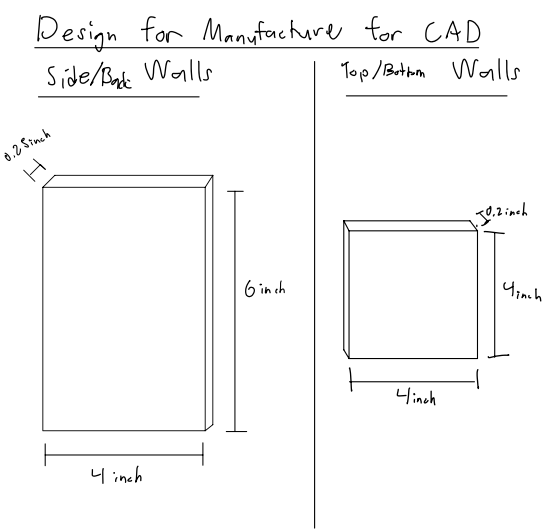
\includegraphics[width=0.8\linewidth]{img/DFM_Side_and_top_wall.png}
    % \caption{Physical Solution Chart}
    \label{fig:enter-label}
\end{figure}
\newpage % This is a new section

\subsection{\textcolor{gray}{Outstanding Issues}}
\textcolor{teal}{\textbf{Hardware/Physical}}
\begin{itemize}
    \item Need to find solenoid lock compatible with ESP32-C3 for testing
    \item Need to make sure generated and customized PINs work with hardware authorization/verification within physical keypad
     \item Need to find battery pack with lifespan of 1.5yrs+
     \item Need to find keypad that can be wired securely to ESP32-C3 in lock 
\end{itemize}
\textcolor{teal}{\textbf{Software/Online}}
\begin{itemize}
     \item Need to print and ensure CAD design works using 123A printers
     \item Programming correct PIN interface storage with secure random generation
     \item 
    
\end{itemize}

\section{Appendices}

\textcolor{teal}{\subsection{Brainstorming Ideas}} \label{BrainstormingIdeas}

\subsubsection{6-3-5 Method}
\subsubsection*{Hardware \& Mechanics}
\begin{itemize}
    \item use a servo motor for deadbolt control
    \item hall effect sensor to detect if the door is open or closed
    \item implement linear actuator for silent locking
    \item maybe anti-backlash gears to reduce mechanical play
    \item consider designing a modular lock housing with 3D-printed parts
    \item have a backup battery to ensure operation during power outages
\end{itemize}

\subsubsection*{Smartphone Integration}
\begin{itemize}
    \item develop a smartphone app for remote locking/unlocking
    \item push notifications for lock activity (ex: ``Door locked at 3:45 PM'')
    \item have biometric authentication (Face ID or fingerprint)
    \item Use Bluetooth for proximity-based auto-unlock
    \item NFC support for quick unlocking via phone tap
    \item include multi-user access control with time-based permissions
\end{itemize}

\subsubsection*{Security Features}
\begin{itemize}
    \item Implement AES-256 encryption for communication between the lock and phone
    \item maybe two-factor authentication for app access
    \item develop a tamper-detection alarm if the lock is forced
    \item lockdown mode for multiple failed attempts
    \item include a manual override mechanism in case of system failure
    \item utilize rolling codes for Bluetooth pairing to prevent hacking
\end{itemize}

\subsubsection*{Software \& Control}
\begin{itemize}
    \item ESP32 microcontroller for Wi-Fi and Bluetooth control
    \item Develop a closed-loop system to verify if the lock is engaged properly
    \item make a real-time event log accessible via the app
    \item add a scheduling feature for auto-locking at specific times
    \item guest mode with temporary passcodes
    \item Integration with voice assistants like Alexa or Google Assistant
\end{itemize}

\subsubsection*{Advanced Features}
\begin{itemize}
    \item GPS stuff
    \item add geofencing to lock or unlock based on the user's location
    \item integrate with smart home platforms like Home Assistant
    \item use AI-based behavior analysis to suggest locking patterns
    \item add a camera with facial recognition for auto-unlock
    \item enable remote firmware updates
    \item learn database SQL
    \item use solar charging for battery-powered locks
\end{itemize}

% BRAINSTORMING -----------------------------

\subsubsection{Brainstorming}

\subsubsection*{Adam Wu}
\begin{itemize}
    \item As a person who has amnesia, I would like to be able to find my keys anytime so that when I forget where I place them, I can find them.
    \begin{itemize}
        \item Having a "find my" solution with a key.
    \end{itemize}
    \item As a person who loves security, I would like to have the best lock for my house so that lock pickers are not able to pick my lock.
    \begin{itemize}
        \item Making an “authentication” key that resets the key code within a set time, making it harder for hackers to unlock the door.
    \end{itemize}
    \item As a person who is always last-minute out the door, I fear forgetting to lock the door when I close it.
    \begin{itemize}
        \item Auto-locking door when a person closes the door.
    \end{itemize}
    \item As a person who often forgets to bring their keys, I am scared of getting locked out.
    \begin{itemize}
        \item Having a notification from the key to the phone that alerts: “keys are not close by to you.”
    \end{itemize}
    \item As a parent, I am scared of my kids forgetting their keys and locking themselves out of their room.
    \begin{itemize}
        \item Creating a “master key” that only parents/admins can use to unlock specific doors.
    \end{itemize}
    \item Concerned about key battery life.
    \begin{itemize}
        \item Send a notification to the user when the key is on low battery.
    \end{itemize}
\end{itemize}

\subsubsection*{Nathaniel Laurente}
\begin{itemize}
    \item Key has the ability to notify the user when too far away from the user’s phone/body.
    \item Key deactivates/won’t be able to open the door if too far away from the owner.
    \item “Tap to Pay” technology concept.
    \begin{itemize}
        \item Unlocks the door like a credit card tap on a phone.
        \item If too complex, explore alternative ways to unlock the door.
        \item Eliminates the need for a physical key.
        \item Prevents stolen keys from working if the user still has their phone.
    \end{itemize}
    \item Secure deactivation of the key when too far from the user.
    \begin{itemize}
        \item Possible solution: Use the user's phone for deactivation.
    \end{itemize}
    \item One-time password generator between lock and key to ensure only this exact key can enter the house.
    \item Backup way to get into the house if the user forgets/loses their key.
    \begin{itemize}
        \item Pin access code.
        \item App allows for 2FA authentication using a thumbprint and/or Face ID.
    \end{itemize}
    \item Will the battery last long enough for multiple years?
\end{itemize}

\subsubsection*{Neena Nguyen}
\begin{itemize}
    \item Existing smart lock solutions:
    \begin{itemize}
        \item Smart locks for dorm rooms using mobile apps, passcodes, and scanners.
    \end{itemize}
    \item Who will use this lock?
    \begin{itemize}
        \item People with memory issues (elderly, ADHD).
        \item University students in dorm rooms.
        \item Student ID scanner integration.
        \item Parents with small children (child-proof locks).
    \end{itemize}
    \item Features for parental control.
    \begin{itemize}
        \item Locks after a curfew time.
        \item Prevents children from unlocking without parental approval.
        \item Alerts parents when kids come home from school.
    \end{itemize}
    \item What kind of door lock will it be?
    \begin{itemize}
        \item Facial recognition (requires camera and database knowledge).
        \item Logs entry and exit timestamps.
        \item Digital passcode through an app.
        \item Auto-relocking mechanism after failed attempts.
        \item Bluetooth detection for unlocking within a certain range.
        \item Dual authentication (PIN + scan).
        \item Optional security trigger after specific hours.
        \item Alerts when the door is left unlocked for too long.
        \item Auto-locking after prolonged unlocking.
        \item Detection system to check if the key is on the person.
        \item Prevents intruders from entering without a key.
    \end{itemize}
\end{itemize}

\subsubsection*{Jackson Kennedy}
\begin{itemize}
    \item Normal keys can be lock-picked, but digital keys can be secured based on a communication protocol.
    \item Secure authentication methods.
    \begin{itemize}
        \item PIN authentication with 2FA.
        \item Optimal PIN length (e.g., 4-digit PIN has 1,048,576 combinations).
        \item Brute force prevention strategies.
    \end{itemize}
    \item Preventing communication protocol vulnerabilities.
    \begin{itemize}
        \item What protocol should be used? (Bluetooth has vulnerabilities and short range.)
        \item Cloud-based solutions rely on third-party vendor security.
        \item What information needs to be transferred? (Video data, authentication signals?)
    \end{itemize}
    \item Lock activation logic.
    \begin{itemize}
        \item How exactly will the lock know when to unlock? (Sending a 0 or 1 signal based on specific conditions?)
    \end{itemize}
    \item Security and alerting technologies.
    \begin{itemize}
        \item Sensors to detect nearby people.
        \item Hidden camera or biometric verification for identity confirmation.
    \end{itemize}
    \item Scheduling and timed access.
    \begin{itemize}
        \item Physical locks do not have scheduling options.
        \item Implement timed unlocking (e.g., unlock for 15 minutes for a babysitter).
        \item Extra verification to prevent intruders from exploiting schedules.
    \end{itemize}
\end{itemize}
\newpage

% Begin Morphological Charts ----------------------------------

\subsubsection{Morphological Charts}

\begin{figure}[!ht]
    \centering
    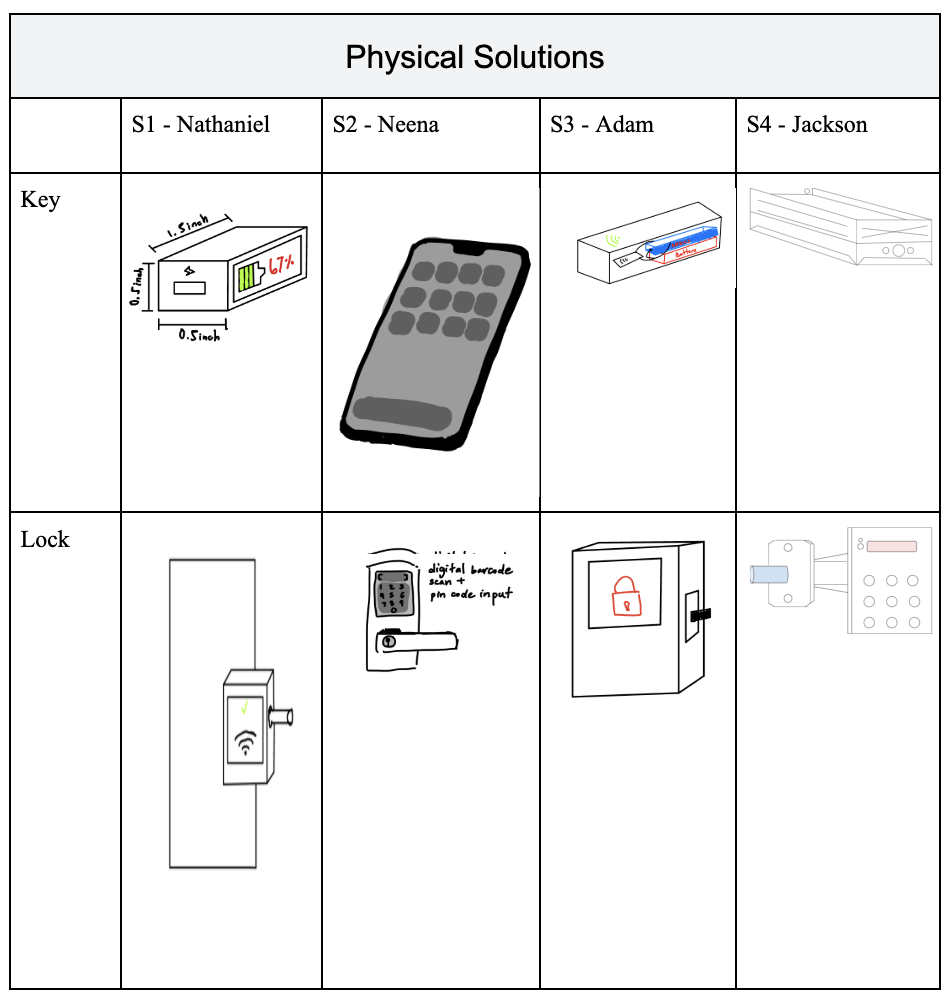
\includegraphics[width=1\linewidth]{./img/p1mm.png}
    \caption{Physical Solution Chart}
    \label{fig:p1mm}
\end{figure}
\newpage
\begin{figure}[!ht]
    \centering
    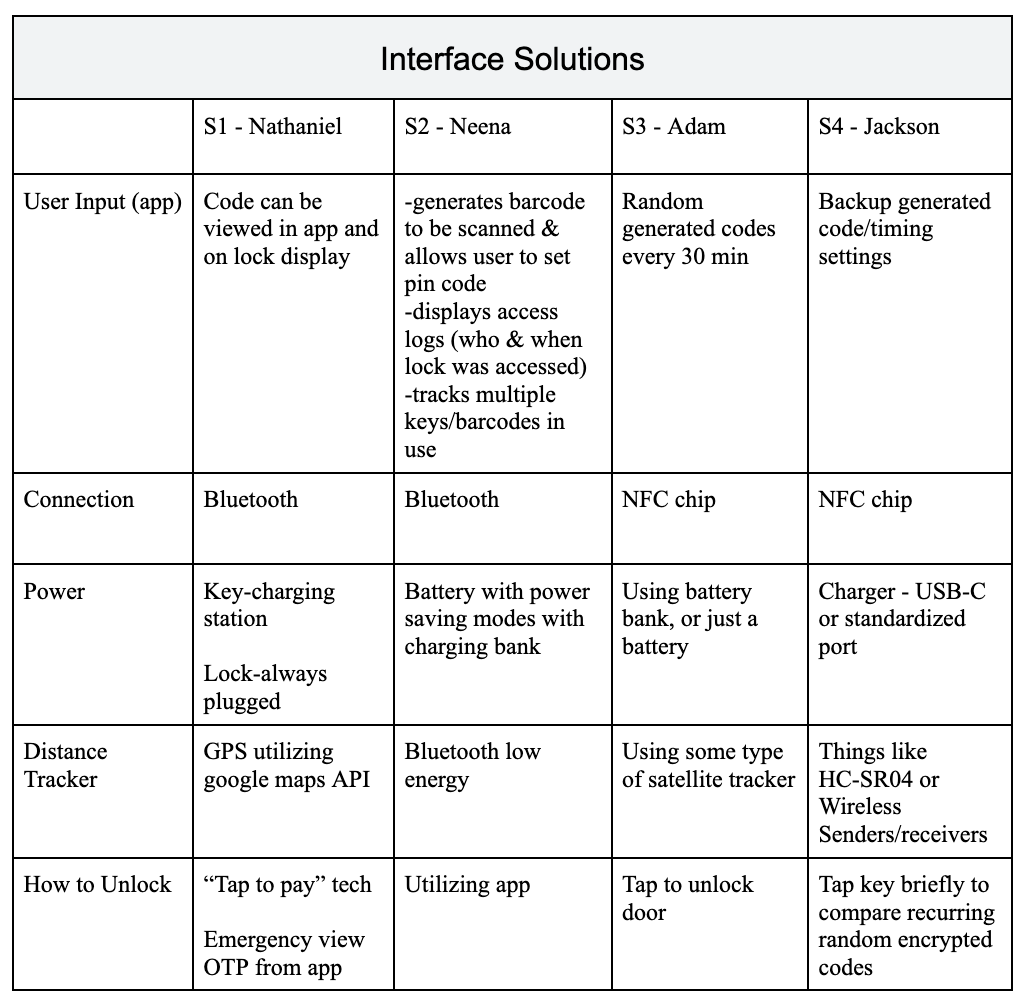
\includegraphics[width=1\linewidth]{./img/p2mm.png}
    \caption{Interface Solutions}
    \label{fig:p2mm}
\end{figure}
\newpage

% Begin Mind Map ---------------------------------------------

\subsubsection{Mind Map}

\begin{figure}[!ht]
    \centering
    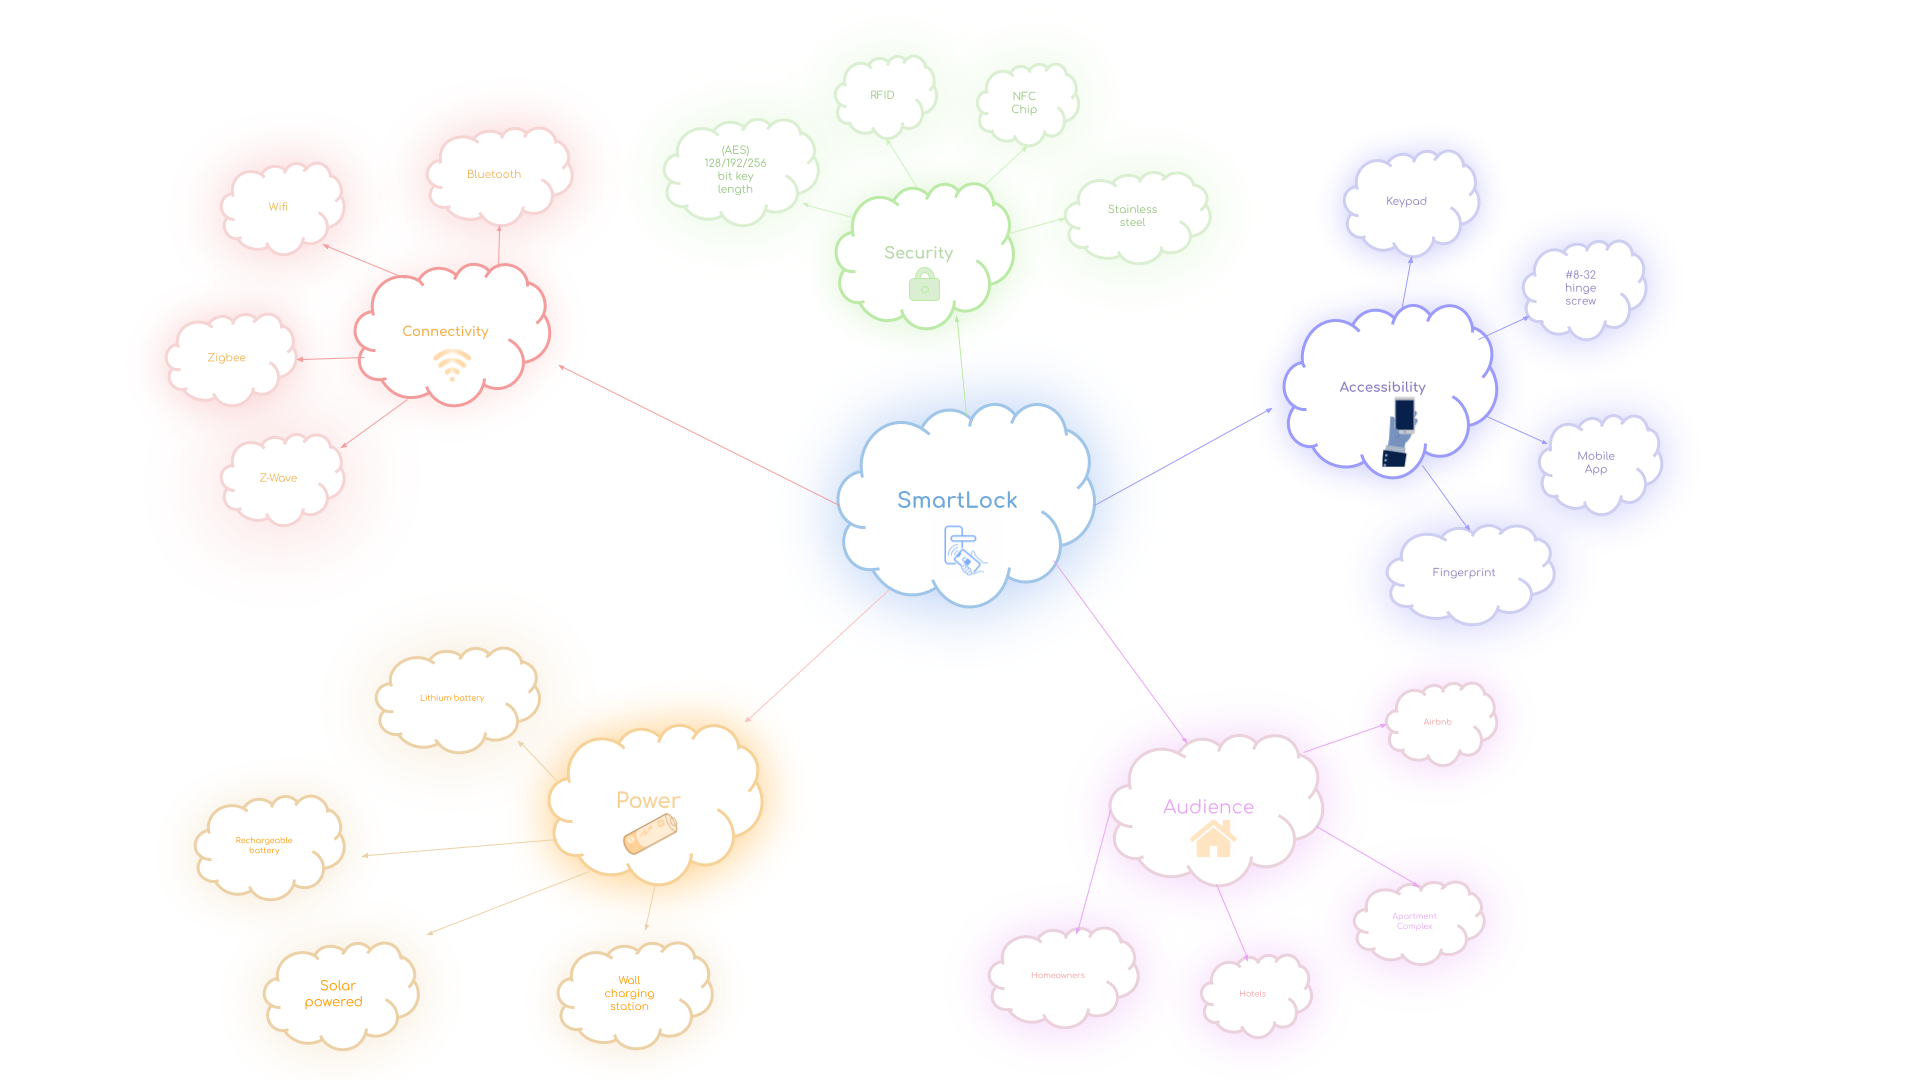
\includegraphics[width=140mm,scale=0.5]{./img/mindmapsmartlock.png}
    \caption{Mind Map}
    \label{fig:mindmapsmartlock}
\end{figure}

\subsubsection{Concept Selection}
\subsubsection*{Weighting Factors}
\begin{tabular}{ll}
    \toprule
    Criteria & Weight (\%) \\
    \midrule
    Security & 40 \\
    Cost & 30 \\
    Power Consumption & 20 \\
    User Convenience & 10 \\
    \textbf{Total} & \textbf{100} \\
    \bottomrule
\end{tabular}

\subsubsection*{Decision Table}
\resizebox{\textwidth}{!}{%
\begin{tabular}{lcccc}
    \toprule
    Criteria & Weight & Design 1 (Basic) & Design 2 (Mid-Range) & Design 3 (Advanced) \\
    \midrule
    Security & 40 & 6 (240) & 8 (320) & 10 (400) \\
    Cost & 30 & 10 (250) & 6 (150) & 3 (75) \\
    Power Consumption & 20 & 6 (90) & 8 (120) & 10 (150) \\
    User Convenience & 10 & 3 (30) & 6 (60) & 9 (90) \\
    \textbf{Total Score} & \textbf{100} & \textbf{680} & \textbf{720} & \textbf{780} \\
    \bottomrule
\end{tabular}%
}

\textbf{Best Design:} Design 3 (Advanced) with 780 points, prioritizing security, cost-efficiency, and power optimization.


\textcolor{teal}{\subsection{Scope}}
\subsubsection*{Firebase Mobile Connectivity Test}
\subparagraph{Test Goals and Purpose}
\begin{itemize}
    \item Ensure that an IOS device can securely connect and push data to the Firebase Firestore servers.
    \item What happens when there may be bad network connection
    \item Set a certain time frame for the pin to be qualified for
\end{itemize}

\subparagraph{Parameters}
\begin{itemize}
    \item 1/0 LOCK$\_$STATE necessary for defining lock-state, 1 is unlocked, 0 is locked.
    \item 7 digit QUALIFIED$\_$PIN list on an allow list for physical keypad on SmartLock.
    \item Make sure what data we send from phone is on firebase
    \item Provide time frame as input for start and expiration time for pin code
\end{itemize}

\subparagraph{Expectations of Test}
\begin{itemize}
    \item There will be no issue with pushing a simple piece of data for LOCK$\_$STATE to the firestore servers, clicking lock will properly push a 0 and clicking unlock will store a 1. Additionally, the pin list composed of generated and custom user pins will also have no trouble being communicated with Firestore servers to later be fetched by the physical device as an additional mechanism for locking and unlocking.
    \item Testing the time frame of the pin code, ensure only the time when valid to use the pin. Otherwise other times should be invalid.
\end{itemize}

\subsubsection{Lock Hardware Functionality Test}
\subparagraph{Test Goals and Purpose}
\begin{itemize}
    \item Ensure that an ESP32-C3 device can securely connect and retrieve data from the Firebase Firestore servers.
    \item Ensure that the ESP32-C3 board can correctly interact with hardware to enable mechanisms for locking/unlocking.
    \item Ensure that invalid codes should not release bolt, while valid codes should.
\end{itemize}


\subparagraph{Parameters}
\begin{itemize}
    \item 1/0 LOCK$\_$STATE necessary for defining lock-state, 0 is locked, 1 is unlocked. Retrieved from firebase.
    \item 7 digit QUALIFIED$\_$PIN list on an allow list for physical keypad on SmartLock.
\end{itemize}

\subparagraph{Expectations of Test}
\begin{itemize}
    \item The locking mechanism will respond appropriately after retrieving from Firestore, and the bolt will trigger when the parameter is set to 0 and likewise release given a 1 value. Additionally, the bolt will release given a valid input from the QUALIFIED$\_$PIN list and reject other non-valid input pins.
    \item Expecting the lock to not unlock after a code is expired, only unlock when it is still valid in a time frame.
\end{itemize}

\subsubsection{Multi-User \& Concurrency Test (Low Priority)}
\subparagraph{Test Goals and Purpose}
\begin{itemize}
    \item Ensure that multiple users can simultaneously interact with the smart lock through the mobile app and keypad without causing system conflicts.
    \item Verify that Firebase can handle concurrent updates to the lock state and PIN list without failure.
    \item Ensure the lock responds appropriately when multiple unlock requests are received from different users.
\end{itemize}


\subparagraph{Parameters}
\begin{itemize}
    \item Simultaneous requests from different mobile devices attempting to unlock/lock the door.
    \item Simultaneous PIN entries from different users on the physical keypad and mobile app.
\end{itemize}

\subparagraph{Expectations of Test}
\begin{itemize}
    \item Multiple users attempting to unlock the door at the same time should not cause conflicts or undefined behavior.
    \item The lock should process and execute the most recent valid request, ensuring no delays or duplicate actions.
    \item System logs should correctly track each user’s request, ensuring accountability and reliable data collection for user feedback.
\end{itemize}
\newpage

% New Section ----------------------------------------------------------------------------------------
\textcolor{teal}{\subsection*{Administrative Details}}

\subsubsection{Firebase Mobile Connectivity Test}
\textbf{\textit{Date $\&$ Location:}} Mar 12, 2025 in class
\newline
\textbf{\textit{Conducting Test:}} Jackson Kennedy, Adam Wu, Nathaniel Laurente, Neena Nguyen, and Professor Harrison.

\subsubsection{Lock Hardware Functionality Test}
\textbf{\textit{Date $\&$ Location:}} Mar 31, 2025 in class
\newline
\textbf{\textit{Conducting Test:}} Jackson Kennedy, Adam Wu, Nathaniel Laurente, Neena Nguyen, and Professor Harrison.

\subsubsection{Multi-User \& Concurrency Test}
\textbf{\textit{Date $\&$ Location:}} April 18, 2025 in class
\newline
\textbf{\textit{Conducting Test:}} Jackson Kennedy, Adam Wu, Nathaniel Laurente, Neena Nguyen, and Professor Harrison.

\textcolor{teal}{\subsection*{Design of Experiment}}
\subsubsection{Firebase Mobile Connectivity Test}
\textbf{\textit{Testing method type:}} Functional Testing, does the simple job of sending unlock or lock to firebase server, also sending pins.
\newline
\textbf{\textit{Test apparatus:}} Firebase Cloud service
\newline
\textbf{\textit{Independent Variables:}} Lock Status, Acceptable Pins
\newline
\textbf{\textit{Dependent Variables:}} N/A
\newline
\textbf{\textit{Number of factors:}}
\newline
\textbf{\textit{Sampling Procedures:}} 2 samples of observing Firestore for 1/0 LOCK$\_$STATE. 2 randomly generated PINs and 1 custom-user pin.

\subsubsection{Lock Hardware Functionality Test}
\textbf{\textit{Testing method type:}} When phone sends data for unlock or lock onto firebase, the lock should quickly retrieve information and respond accordingly. The purpose of this is to make sure the lock receives the data fast enough so that people waiting outside the lock does not wait too long for door to unlock. This should also be similar for the pin code case.
\newline
\textbf{\textit{Test apparatus:}} Utilize ESP32-C3 alongside a Solenoid door lock.
\newline
\textbf{\textit{Independent Variables:}} Make sure that the ESP32-C3 can read a simple "Hello world" on the server for basic testing.
\newline
\textbf{\textit{Dependent Variables:}} Everytime we are generating a new code from phone to firebase, the ESP32-C3 should also be able to retrieve those codes as valid codes immediately.
\newline
\textbf{\textit{Number of factors:}} N/A factors considered in this moment
\newline
\textbf{\textit{Sampling Procedures:}} Samples obtained from servers for LOCK\_STATE, only 0 or 1. Then we have samples for pin codes as well from Firebase.
\newline

\subsubsection{Multi-User \& Concurrency Test}
\textbf{\textit{Testing method type:}} Multiple phones will send an unlock signal from phone at nearly the exact same time and see if any undefined behavior occurs. Send a lock signal and an unlock signal at the same time to test if we can prioritize actions that came first, or lock the app after an action from one device has been made.
\newline
\textbf{\textit{Test apparatus:}} Mobile Device along with ESP32-C3.
\newline
\textbf{\textit{Independent Variables:}} Make sure that the ESP32-C3 can read a simple "Hello world" on the server for basic testing.
\newline
\textbf{\textit{Dependent Variables:}} ESP32-C3 behavior after multiple devices send a signal at the same time or immediately one after the other.
\newline
\textbf{\textit{Number of factors:}} 2 factors to be considered
\newline
\textbf{\textit{Sampling Procedures:}} Samples obtained from servers for LOCK\_STATE, only 0 or 1. Determine if multiple signals causes undefined or expected behavior.



\textcolor{teal}{\subsection*{Testing Procedures}}
\subsubsection{Safety Precautions}
Safety precautions for our project includes not having fast and forceful locks that can hurt individuals.

\subsubsection{Data Collection Method}
Collect data from the phone providing the custom pins onto firebase, as well as collecting data for locking or unlocking. We will also note down which users are grouped together to be able to use the same pin for unlcocking door.

\subsubsection{Observation of External Factors}
Some external factors that could make our product not function properly could include:

\begin{itemize}
    \item Bad network connection from phone or from ESP32-C3
    \item Firebase not loading properly
\end{itemize}

\subsection{Test Results}

\subsubsection{From Test Plan}
We will be testing our Firebase mobile connectivity, Esp32 hardware functionality, and multi-user and concurrency. For each of the tests, I will provide step by step instructions.

In the first test for Firebase mobile connectivity, we will test the connection between the mobile app and the firestore database. We will first build the mobile app and connect the firebase API keys to the app. Then with the mobile app, we will test the connection to the firestore database by sending a value to the database document. We can check if this succeeds by checking the firebase console and seeing if the value is updated.

In the second test for the ESP32 hardware functionality, we will test the connection between the ESP32 and wifi. Once connected to wifi, we will test the connection to the firestore database by using the API keys provided by firebase. Then we will create a document in the firestore database and use the ESP32 to fetch the document data. We can check if this succeeds by checking the fetched data is the same as the data in the firestore database. Also from the hardware functionality test, we are going to test the functionality of the solenoid lock, making sure that we can send a signal to unlock and lock the solenoid lock. One more test that we will need to take into consideration is the keypad functionality. We will test the functionality of the keypad by making sure that we can read the input from the keypad and send the input to the ESP32.

In the third test for multi-user and concurrency, we will test the connection between multiple mobile apps and the firestore database. We will first build the mobile app and connect the firebase API keys to the app. Then with the mobile app, we will test the connection to the firestore database by sending a value to the database document. We can check if this succeeds by checking the firebase console and seeing if the value is updated. We will then test the connection between multiple mobile apps and the firestore database by sending values to the database document from multiple mobile apps. We can check if this succeeds by checking the firebase console and seeing if the values are updated.

% GPT table
\subsubsection{Test Result Summary Table}
\begin{table}[h]
    \centering
    \resizebox{\textwidth}{!}{ % Resizes table to fit within page width
    \rowcolors{2}{teal!10}{teal!25}
    \begin{tabular}{|l|c|c|p{6cm}|}
        \hline
        \rowcolor{teal!50}
        \textbf{Objective ( Target )} & \textbf{Result} & \textbf{Met?} & \textbf{Discussion} \\
        \hline
        Firebase Connectivity & Appropriate 1/0 & N/A & Half this test done - explain how lock/unlock work but haven't tested PINs yet. \\
        
        Lock Hardware Functionality & N/A -\textit{Mar 31, 2025} & N/A & While this test has not been conducted yet, we suspect we will pass this test as the Firebase - Firestore lock/unlock was already successful, and the appropriate data was well-received by the ESP32-C3. All that remains is to ensure that the solenoid lock responds properly to an input signal, as well as compares and responds accordingly to valid/invalid codes. \\
        
        Concurrency & N/A -\textit{April 18, 2025} & N/A & While this test has not been conducted yet, we suspect that we will pass this test. Firebase should be able to handle multiple calls close to each other, as well as transmit this signal in the appropriate order. The Firestore database updated extremely quickly in real-time and shouldn't have trouble with concurrent calls. The PIN entries from different users also shouldn't cause conflict, and the door should unlock/lock as intended. \\
        
        \hline
    \end{tabular}}
\end{table}


\newpage
\begin{samepage}
    \section{Manufactured Product Testing}
    \subsection{Common Scenarios (Tests 1–10)}
% ---------------------------- Test 1 --------------------------------
    \subsection*{1. Valid PIN Entry Test}
    \subparagraph{Test Goals and Purpose}
    \begin{itemize}
        \item Verify that a recognized 4-digit PIN unlocks the door without unnecessary delay.
        \item Check that the system logs this event as a successful access in Firestore.
    \end{itemize}
    \subparagraph{How We Test It}
    \begin{enumerate}
        \item Select a PIN known to be valid from the internal list.
        \item Enter the PIN once on the keypad.
        \item Observe the system's response, checking for physical bolt movement and UI changes on the mobile application.
        \item Look for updates to the (\texttt{LOCK\_STATE}) value in Firestore.
    \end{enumerate}
    
    \textbf{Expectations of Test}
    \begin{center}
    \begin{tabular}{|c|p{10cm}|}
      \hline
      \textbf{Result} & \textbf{Conditions} \\
      \hline
      PASS & Bolt retracts within \textless{}0.5\,s; \texttt{LOCK\_STATE}=1; Firestore log entry \emph{success}. \\
      \hline
      FAIL & Any deviation from the above timing, state, or logging behaviour. \\
      \hline
    \end{tabular}
    \end{center}
\end{samepage}


% ---------------------------- Test 2 --------------------------------
\newpage
\subsection*{2. Invalid PIN Lockout Test}
\subparagraph{Test Goals and Purpose}
\begin{itemize}
    \item Ensure the system prevents further PIN attempts after multiple consecutive failures.
    \item Lock should be shut down for a short expiration period.
    \item Confirm some form of lockout indication is presented, such as a light or warning beep.
    \item Owner's phoone should receive an alert about the failed attempts.
\end{itemize}
\subparagraph{How We Test It}
\begin{itemize}
    \item Enter three clearly incorrect PINs in under 30 seconds.
    \item Observe for a visible or audible signal.
    \item Confirm that \texttt{LOCKOUT\_COUNT} has risen and \texttt{LOCK\_STATE} is still 0 (locked).
\end{itemize}
\subparagraph{Expectations of Test}
\begin{center}
\begin{tabular}{|c|p{10cm}|}
  \hline
  \textbf{Result} & \textbf{Conditions} \\
  \hline
  \textbf{PASS} &
    \begin{minipage}[t]{\linewidth}
    \begin{itemize}
      \item Keypad flashes red and/or beeps immediately after the \textbf{third} wrong entry.
      \item No further PINs are accepted for the lockout period (default: 60 s).
      \item Mobile app log shows “3 invalid PIN attempts – lock is temporarily disabled” within 5 s.
      \item Firestore records \texttt{LOCKOUT\_COUNT = 3} and \texttt{LOCK\_STATE = 0}.\\
    \end{itemize}
    \end{minipage} \\ 
  \hline
  \textbf{FAIL} & Any one of the PASS conditions is missing or incorrect. \\ 
  \hline
\end{tabular}
\end{center}
\vspace{0.5em}

\noindent\textbf{Reset after the test:}  
Either wait for the lockout timer to expire or enter an admin PIN to clear the lockout so the next test starts from a clean state.\\


% ---------------------------- Test 3 --------------------------------
\newpage
\begin{samepage}
    \subsection*{3. Emergency PIN Test}
    \subparagraph{Test Goals and Purpose}
    

\subsection*{4. OTP Entry Test}
\subparagraph{Test Goals and Purpose}
\begin{itemize}
    \item Confirm that an app-generated one-time password (OTP) grants access as expected.
    \item Ensure the OTP mechanism is time-bound and secure against reuse.
\end{itemize}
\subparagraph{How We Test It}
\begin{itemize}
    \item Request a 5-minute valid OTP from the app.
    \item Enter the OTP using the keypad.
    \item Monitor the system and database for changes.
\end{itemize}
\subparagraph{Expectations of Test}
\begin{itemize}
    \item Firestore captures the OTP with a clear expiry time.
    \item Valid OTPs allow immediate unlock.
    \item Expired or incorrect OTPs are properly rejected with no unlock attempt.
\end{itemize}

\subsection*{5. OTP Expiry Test}
\subparagraph{Test Goals and Purpose}
\begin{itemize}
    \item Ensure expired OTPs don’t grant access, even if they were once valid.
    \item Confirm that users are informed clearly when an OTP is no longer usable.
\end{itemize}
\subparagraph{How We Test It}
\begin{itemize}
    \item Generate an OTP and wait for the full 5-minute window to pass.
    \item Attempt to use the expired code via the keypad.
\end{itemize}
\subparagraph{Expectations of Test}
\begin{itemize}
    \item Lock remains unchanged and secure—no movement or unlock occurs.
    \item Firestore logs the expired OTP attempt explicitly.
    \item App and/or interface display an "OTP expired" notification.
\end{itemize}

\subsection*{6. Rapid Wrong PIN Alarm Test}
\subparagraph{Test Goals and Purpose}
\begin{itemize}
    \item Ensure multiple fast wrong PIN entries trigger audible alarm.
    \item Verify lock does not unlock after wrong entries.
    \item Check alarm stops after timeout or correct PIN.
\end{itemize}
\subparagraph{How We Test It}
\begin{itemize}
    \item Enter 5 wrong PINs within 10s.
    \item Observe alarm sound and LOCK\_STATE remains 0.
    \item Attempt correct PIN after alarm to confirm reset.
\end{itemize}
\subparagraph{Expectations of Test}
\begin{itemize}
    \item Alarm beeps continuously for spec duration (e.g., 30s).
    \item Bolt remains locked (LOCK\_STATE = 0).
    \item Firestore logs each failed attempt and alarm event.
    \item Correct PIN after alarm silences alarm and unlocks door.
\end{itemize}

\subsection*{7. Concurrent Unlock Command Test}
\subparagraph{Test Goals and Purpose}
\begin{itemize}
    \item Verify two family phones sending unlock at once doesn't confuse the system.
    \item Ensure only one actuation happens.
    \item Confirm both requests are logged.
\end{itemize}
\subparagraph{How We Test It}
\begin{itemize}
    \item From two phones, send unlock API calls within 100 ms.
    \item Watch bolt movement and LOCK\_STATE.
    \item Check Firestore for two event entries.
\end{itemize}
\subparagraph{Expectations of Test}
\begin{itemize}
    \item Bolt retracts only once.
    \item LOCK\_STATE = 1 after first command.
    \item Both commands logged with timestamps.
    \item No errors or retries triggered.
\end{itemize}

\subsection*{8. Offline Fallback PIN Test}
\subparagraph{Test Goals and Purpose}
\begin{itemize}
    \item Ensure local PIN entry still works if Wi-Fi drops.
    \item Verify lock uses cached PIN list.
    \item Confirm Firestore syncs later.
\end{itemize}
\subparagraph{How We Test It}
\begin{itemize}
    \item Disable Wi-Fi on ESP32, enter valid PIN.
    \item Observe bolt movement and local log.
    \item Re-enable Wi-Fi and check Firestore sync.
\end{itemize}
\subparagraph{Expectations of Test}
\begin{itemize}
    \item Door unlocks locally (LOCK\_STATE = 1 locally).
    \item Event cached and later pushed to Firestore.
    \item No user-perceived delay in unlocking.
    \item Sync event marked with “offline” flag.
\end{itemize}

\subsection*{9. Low-Battery Notification Test}
\subparagraph{Test Goals and Purpose}
\begin{itemize}
    \item Check notification when battery falls below 10 %.
    \item Ensure unlock still works at low battery.
    \item Verify UI warning persists until charge.
\end{itemize}
\subparagraph{How We Test It}
\begin{itemize}
    \item Drain battery to 9 %.
    \item Press unlock PIN and observe behavior.
    \item Check mobile app for low-battery alert.
\end{itemize}
\subparagraph{Expectations of Test}
\begin{itemize}
    \item Door still unlocks (LOCK\_STATE = 1).
    \item App shows persistent “Low Battery” message.
    \item Firestore logs battery level event.
    \item Warning clears only when battery > 20 %.
\end{itemize}

\subsection*{10. Battery Fully Drained Test}
\subparagraph{Test Goals and Purpose}
\begin{itemize}
    \item Verify lock fails to actuate when battery is dead.
    \item Ensure system logs failure and alerts user.
    \item Confirm physical key still works.
\end{itemize}
\subparagraph{How We Test It}
\begin{itemize}
    \item Let battery drop to 0\%.
    \item Enter valid PIN and observe no bolt movement.
    \item Try physical key override.
\end{itemize}
\subparagraph{Expectations of Test}
\begin{itemize}
    \item Bolt does not move on electronic command.
    \item Firestore logs “Battery Depleted” error.
    \item Physical key unlocks door.
    \item App advises “Replace Battery” notification.
\end{itemize}


\subsection*{11. Battery Fully Drained Test}
\subparagraph{Test Goals and Purpose}
\begin{itemize}
    \item Verify lock fails to actuate when battery is dead.
    \item Ensure system logs failure and alerts user.
    \item Confirm physical key still works.
\end{itemize}
\subparagraph{How We Test It}
\begin{itemize}
    \item Let battery drop to 0 \%.
    \item Enter valid PIN and observe no bolt movement.
    \item Try physical key override.
\end{itemize}
\subparagraph{Expectations of Test}
\begin{itemize}
    \item Bolt does not move on electronic command.
    \item Firestore logs “Battery Depleted” error.
    \item Physical key unlocks door.
    \item App advises “Replace Battery” notification.
\end{itemize}

























\newpage
\subsection{Less Common Scenarios (Tests 31–40)}

\subsection*{31. Multi-factor Auth Proximity Test}
\subparagraph{Test Goals and Purpose}
\begin{itemize}
    \item Confirm the system requires both a valid PIN and Bluetooth proximity to unlock.
    \item Observe behavior if Bluetooth disconnects mid-process.
\end{itemize}
\subparagraph{How We Test It}
\begin{itemize}
    \item Start PIN entry and slowly move the paired phone out of Bluetooth range.
    \item Review logs to see how the system treats incomplete multi-factor input.
\end{itemize}
\subparagraph{Expectations of Test}
\begin{itemize}
    \item Door only unlocks when both factors are simultaneously validated.
    \item Firestore logs clearly show whether it was the PIN or BLE that failed.
\end{itemize}

\subsection*{32. Time-zone Mismatch Test}
\subparagraph{Test Goals and Purpose}
\begin{itemize}
    \item Ensure that timing-sensitive operations work properly despite device time mismatches.
    \item Verify that scheduled actions and OTPs remain aligned regardless of local time zones.
\end{itemize}
\subparagraph{How We Test It}
\begin{itemize}
    \item Set the phone to Pacific Time and the lock to Coordinated Universal Time.
    \item Generate and use an OTP, and observe if the mismatch causes issues.
\end{itemize}
\subparagraph{Expectations of Test}
\begin{itemize}
    \item OTPs still work during their intended validity window.
    \item Scheduled events (e.g., auto-lock) trigger based on synchronized absolute times.
\end{itemize}

\subsection*{33. DST Transition Auto-lock Test}
\subparagraph{Test Goals and Purpose}
\begin{itemize}
    \item Confirm that daylight saving time transitions don't disrupt automated locking.
\end{itemize}
\subparagraph{How We Test It}
\begin{itemize}
    \item Schedule an auto-lock event for 2:00 AM on the day of the DST shift.
    \item Observe actual lock behavior before, during, and after the transition.
\end{itemize}
\subparagraph{Expectations of Test}
\begin{itemize}
    \item Only one auto-lock event occurs, even with the clock shift.
    \item No skipped or duplicated scheduling happens.
\end{itemize}

\subsection*{34. Admin vs. Guest Role Change Test}
\subparagraph{Test Goals and Purpose}
\begin{itemize}
    \item Validate that role-based access control takes effect immediately after role changes.
\end{itemize}
\subparagraph{How We Test It}
\begin{itemize}
    \item Change a user's role (e.g., from guest to admin) directly in Firestore.
    \item Attempt access under both roles shortly after the change.
\end{itemize}
\subparagraph{Expectations of Test}
\begin{itemize}
    \item The new role is honored without requiring system restart or delay.
    \item Access permissions align with the updated role instantly.
\end{itemize}

\subsection*{35. BLE Range Boundary Test}
\subparagraph{Test Goals and Purpose}
\begin{itemize}
    \item Determine the Bluetooth unlocking behavior at different physical distances.
\end{itemize}
\subparagraph{How We Test It}
\begin{itemize}
    \item Gradually move the phone away from the lock in 0.5-meter steps, from 1 m up to 6 m.
    \item Test unlocking at each position and note the results.
\end{itemize}
\subparagraph{Expectations of Test}
\begin{itemize}
    \item Unlocks reliably at closer distances.
    \item Fails gracefully beyond Bluetooth’s effective range.
\end{itemize}










































\newpage
\subsection{Rare Scenarios (Tests 61–65)}

\subsection*{61. Cosmic Ray Bit-Flip Test}
\subparagraph{Test Goals and Purpose}
\begin{itemize}
    \item Evaluate the system’s resilience to random memory errors, such as those caused by cosmic rays.
\end{itemize}
\subparagraph{How We Test It}
\begin{itemize}
    \item Use a simulator to inject random bit flips into RAM and flash every 10 seconds.
    \item Observe system behavior over an extended period.
\end{itemize}
\subparagraph{Expectations of Test}
\begin{itemize}
    \item System detects and handles bit errors—either by correcting or isolating them.
    \item No persistent crashes or loss of functionality.
\end{itemize}

\subsection*{62. Lightning Surge Test}
\subparagraph{Test Goals and Purpose}
\begin{itemize}
    \item Assess whether the hardware can tolerate sudden electrical surges.
\end{itemize}
\subparagraph{How We Test It}
\begin{itemize}
    \item Apply a 1-kV spike to the 12V input for a 1 microsecond duration using a surge generator.
\end{itemize}
\subparagraph{Expectations of Test}
\begin{itemize}
    \item No hardware is permanently damaged.
    \item System recovers and operates normally after the surge event.
\end{itemize}

\subsection*{63. Seismic Vibration Test}
\subparagraph{Test Goals and Purpose}
\begin{itemize}
    \item Verify the lock’s mechanical and electronic components withstand prolonged shaking.
\end{itemize}
\subparagraph{How We Test It}
\begin{itemize}
    \item Subject the device to a vibration range of 5–50 Hz at 0.5 g for 10 minutes.
    \item Check for loosening, noise, or malfunction.
\end{itemize}
\subparagraph{Expectations of Test}
\begin{itemize}
    \item All parts remain in place and fully operational.
    \item Sensors continue to function accurately post-test.
\end{itemize}

\subsection*{64. Extreme Cold Operation Test}
\subparagraph{Test Goals and Purpose}
\begin{itemize}
    \item Confirm functionality in severe cold conditions down to -40 °C.
\end{itemize}
\subparagraph{How We Test It}
\begin{itemize}
    \item Place the lock in a chamber set to -40 °C for 2 hours.
    \item Perform 10 complete lock/unlock cycles.
\end{itemize}
\subparagraph{Expectations of Test}
\begin{itemize}
    \item Mechanism operates without freezing or delay.
    \item No cracking or material degradation.
    \item Battery and electronics remain reliable.
\end{itemize}

\subsection*{65. Extreme Heat Operation Test}
\subparagraph{Test Goals and Purpose}
\begin{itemize}
    \item Test device reliability when exposed to 85 °C for extended periods.
\end{itemize}
\subparagraph{How We Test It}
\begin{itemize}
    \item Place the lock in a heat chamber at 85 °C.
    \item Execute a lock/unlock cycle every 5 minutes over 2 hours.
\end{itemize}
\subparagraph{Expectations of Test}
\begin{itemize}
    \item No thermal shutdown or malfunctions.
    \item MCU and storage remain intact and responsive.
\end{itemize}



\end{document}